\fenicschapter{Lessons Learned in Mixed Language Programming Using Python, C++ and \swig}
              {Mixed Language Programming}
              {Johan Hake and Kent-Andre Mardal}
              {mixedlanguage}

\section{Introduction}
Python~\cite{www:python} has in the last decade become an established platform for scientific computing. Widely used scientific software like, e.g., \petsc\cite{www:petsc}, \hypre\cite{www:hypre}, \trilinos\cite{pytrilinos}, \vtk\cite{www:vtk}, \itk, \ginac\cite{BauerFrinkEtAl2000} have all been equipped with Python interfaces. In addition many packages like for instance the \fenics packages \ferari, \fiat \cite{Kirby2006}, \ffc\cite{FFC}, \ufl\cite{UFL}, \viper, as well as other packages like \sympy\cite{Sympy}, \scipy\cite{SciPy} are pure Python packages. The \dolfin library has both a C++ and a Python user-interface. Python makes application building on top of \dolfin more user friendly, but the Python interface also introduces additional complexity and new problems. This chapter describes some lessons learned during the development of \pydolfin, and is intentionally quite technical. We assume that the reader has basic knowledge of both C++ and Python. A suitable textbook on Python for scientific computing is \cite{Simula.SC.63}, which cover both Python and its C interface. SWIG is well documented and we refer to the user manual that can be found on its web page~\cite{SWIG}. Finally, we refer to \citet{SC.5.Langtangen.2003.a} and \citet{pytrilinos} for a description of how \swig can be used to generate Python interfaces for Diffpack and Trilinos.\par

All the code examples in this chapter can found in
\emp{\$FENICSBOOK/mixed\_language/}.

\section{Using \swig}
Python and C++ are two very different languages, but they can be glued together as specified by the Python C-API~\cite{www:python-capi}, also see \citet{www:python-extending}. The code that glues together C++ and Python is commonly called wrapper code. Writing wrapper code manually is often cumbersome, therefore wrapper code generators such as e.g. F2PY~\cite{F2Py}, SIP~\cite{SIP}, Siloon~\cite{Siloon}, or \swig~\cite{SWIG} are usually used.  Common for all these code generators are that they create a Python extension module in the form of a shared library. This module can then be imported and accessed as any Python module. \swig has been used to create \pydolfin. \swig is a mature wrapper code generator that support many languages and is extensively documented.\par

\subsection{Basic \swig}
To get a basic understanding of \swig, consider the following definition of an Array class defined in \emp{Array.h}.
\codeinput{chapters/mardal-2/code/Array.h}
A first attempt to make the Array accessible in Python using \swig, is to write a \swig interface file \emp{Array\_1.i}.
\codeinput{chapters/mardal-2/code/Array_1.i}
Here we specify the name of the Python module: \emp{Array}, what code should be inlined directly in the wrapper code (declarations), \emp{\#include "Array.h"} and what code \swig should parse to create the wrapper code \emp{\%include "Array.h"} (definitions). The following command shows how to run \swig on this interface file to produce the wrapper code.
\begin{code}
swig -python -c++ -I. -O Array_1.i
\end{code}
The command generates two files: \texttt{Array.py} and \texttt{Array\_}\texttt{wrap.cxx}. In the file \texttt{Array\_}\texttt{wrap.cxx}, \swig includes everything that is needed to bridge the interface between our C++ class and Python. When \texttt{Array\_wrap.cxx} is compiled into a shared library it can be imported directly into Python, which is done in the generated \texttt{Array.py} file. The file \texttt{Array.py} is  pure python, and in this file \swig has generated code for the so called Python proxy class; a Python version of the C++ defined \texttt{Array} class. The reader should be able to recognize the Python class \texttt{Array} in the end of the \texttt{Array.py} file. \par

The following Distutils file executes the \swig command above and compiles and links the source code and the generated wrapper code into a shared library.
\codeinput{chapters/mardal-2/code/setup.py}
Build and install the module in the current working directory by typing:
\begin{code}
python setup.py install --install-lib=.
\end{code}

The Python proxy class resembles the C++ class in many ways. Simple methods like \emp{dim()} and \emp{norm()} will be wrapped correctly to Python.\footnote{This is because \swig maps int and double arguments to the corresponding Python types through built-in typemaps. \swig also uses typemaps between objects of declared types, like our \emp{Array} class, meaning that the copy constructor will work as expected.} However, there exists a number of corner cases that \swig does not map correctly:
\begin{enumerate}
\item the \emp{operator[]} does not work,
\item the \emp{operator+=} returns a new Python object (with different \texttt{id}),
\item printing does not use the \emp{std::ostream \& operator<<},%>> Put here so emacs highlighting wont go bananas
\item the \emp{Array(int n\_, double* a\_);} constructor is not working properly.%  neither is the overloading of the same method working.
\end{enumerate}
Hence, a number of different problems arise even in such a simple example. Fortunately, these problems are fairly common and simple, and general solutions to these problems can be implemented quite easily. We will go through each of these issues.\par

\subsection{The \texttt{operator[]}}
The first problem is that \swig does not wrap the \texttt{operator[]} from C++ to Python.
One basic observation here is that Python does not have 'const' types. Hence,
the \texttt{operator[]} would in this case be ambiguous\footnote{In general will \swig solve such ambiguities by ignoring one of the methods while issuing a warning.}.
In Python the operator should map to two different special methods: \texttt{\_\_setitem\_\_} and \texttt{\_\_getitem\_\_}. To implement this operator properly, we ignore both version of the \texttt{operator[]} with
\begin{code}
%ignore Array::operator[];
\end{code}
and then tell \swig to extend the C++ extension layer of \texttt{Array} with the mentioned methods. This is done using the \texttt{\%extend} directive.
\begin{code}
%extend Array {
double __getitem__(int i) {
  return (*self)[i];
}

void __setitem__(int i, double v) {
  (*self)[i] = v;
}
...
};
\end{code}
Notice that all \swig directives start with '\texttt{\%}'.
Furthermore, the access to the actual instance is provided by the \texttt{self} pointer, which in this case is a C++ pointer that points to an \texttt{Array} instance. The pointer is comparable to the \texttt{this} pointer in a C++ class, but with only public attributes available. \swig also extends the python proxy class with the same methods.\par

%A basic observation here is that Python does not have \texttt{const} types. This means that if \swig would have wrapped the \texttt{operator[]} methods in the \texttt{Array} class ...
\subsection{\texttt{operator +=} and memory}
The second problem is related to \swig that garbage collection in Python. Python features garbage collection, which means that a user should not be bothered with the destruction of objects. The mechanism is based on reference counting. When no more references are pointing to an object it is destroyed. The \swig generated Python module consists of a small Python layer, that defines the interface to the underlying C++ object. An instance of a \swig generated class therefore keeps a reference to the underlying C++ object. Default behavior is that the C++ object is destroyed together with the Python object. This behavior can be troublesome in quite many cases, which can be illustrated with the following simple example:
\codeinput{chapters/mardal-2/code/segfault_test.py}
This script produce the following output:
\begin{code}
id(a): 3085535980
id(b): 3085535980
id(b): 3085536492
Segmentation fault
\end{code}
The script causes a segmentation fault because the underlying C++ object is destroyed after the call to \texttt{add()}. When the last \texttt{a+=a} is performed there are no C++ object to be added. This happens because the \swig generated \texttt{\_\_iadd\_\_} method returns a new Python object, which will be destroyed in our example. This is illustrated by the different result from the \texttt{id()} function\footnote{Taking \texttt{id} of a Python object returns a unique reference to that object.}. The two calls to \texttt{id(b)} return different numbers, which means that a new Python object is returned by the \swig generated \texttt{\_\_iadd\_\_} method. The variable \texttt{b} is local in the \texttt{add} function. Before the call to \texttt{\_\_iadd\_\_}, \texttt{b} will point to the same Python object as \texttt{a} does; they have the same \texttt{id}. After the call will \texttt{b} point to a new Python object, which is local for the \texttt{add} function. When we leave the function, the reference count to \texttt{b} is decreased to zero and \texttt{b} will be destroyed, together with the underlying C++ object. Therefore, when \texttt{\_\_iadd\_\_} is called at the end of the script, \texttt{a}'s underlying C++ object has been deleted  and we get the segmentation fault.\par

This problem is solved by extending the C++ extension layer with an \texttt{\_add} method, which use the \texttt{operator+=} directly. Furthermore, we extend the Python proxy class with our own \texttt{\_\_iadd\_\_} method that use the \texttt{\_add} function. The following code snippet illustrates the use of \texttt{\%extend}:
\begin{code}
%extend Array {
...
  void _add(const Array& a){
    (*self) += a;
  }

  %pythoncode %{
    def __iadd__(self,a):
      self._add(a)
      return self
  %}
...
};
\end{code}
The same script will report the same \texttt{id} for all objects after the suggested changes has been applied. No objects are created or deleted and we avoid the segmentation fault.\par

\subsection{ \texttt{std::ostream \& operator<<}}%>>
\swig ignores the \texttt{operator <<}, %>>
and this operator is therefore useless from Python. However, we can again use the \texttt{\%extend} directive to make this operator available from Python. We do this by extending the C++ extension layer with a \texttt{\_\_str\_\_} method.
\begin{code}
\begin{code}
%extend Array {
...
  std::string __str__() {
    std::ostringstream s;
    s << (*self);
    return s.str();
  }
};
\end{code}
This method use the \texttt{operator<<} %>>
to pipe the stream representation of array to a \texttt{std::ostringstream} and then return a \texttt{std::string} representation of the stream. To make \swig able to convert a \texttt{std::string} to a Python string, we need to include the \texttt{std\_string.i} file in the \texttt{Array\_2.i} file. In Python we can then call \texttt{print} on an instance of \texttt{Array}, with the result of displaying the content of the \texttt{Array}.\par

\subsection{The constructor: \texttt{Array(int n\_, double* a\_);}}
The fourth problem is related to pointer handling in C/C++ and how \swig deals with pointers.  From the constructor signature alone, it is not clear whether \emp{double *} points to a single value or to the first element of an array.
Therefore, \swig takes a conservative approach and handles pointers as pointers, not assuming anything about the length.
In this example, we do of course know that
\emp{double* a} points to the first element of an array of length \emp{n}.
%In the \emp{Array(int n\_, double* a\_)} constructor, \emp{a\_} is a pointer to the first element in an array of length \emp{n\_}.
However, \swig provides the concept 'typemap' to enable mappings between C/C++ types and Python objects.
The following code demonstrates how to map a Numpy array
to, e.g., the \emp{(int n\_, double* a\_)} constructor.
\begin{code}
%typemap(in) (int n_, double* a_){
  if (!PyArray_Check($input)) {
    PyErr_SetString(PyExc_TypeError, "Not a NumPy array");
    return NULL; ;
  }
  PyArrayObject* pyarray = reinterpret_cast<PyArrayObject*>($input);
  if (!(PyArray_TYPE(pyarray) == NPY_DOUBLE)) {
    PyErr_SetString(PyExc_TypeError, "Not a NumPy array of doubles");
    return NULL; ;
  }
  $1 = PyArray_DIM(pyarray,0);
  $2 = static_cast<double*>(PyArray_DATA(pyarray));
}
\end{code}
A reader not familiar with the C-APIs of Python and \numpy will probably consider this typemap code as fairly technical, but it is a good example as it demonstrates some of the possibilities with typemaps. \par
The first line specifies that the typemap should be applied to input \texttt{(in)} arguments to the C++ library, which has the signature \emp{int n\_,double* a\_}. The \$ prefixed variables are used to map in and output variables in the typemap. The variables \$1 and \$2 maps to the first and second argument of the typemap, i.e., \emp{n\_} and \emp{a\_}. Furthermore, \$input maps to a pointer to the Python object a user is calling the \swig generated method with. \par
In the next three lines we check if the input Python object is a \numpy array, and raise an exception if not.
Note that any Python C-API function that returns \emp{NULL} tells the Python interpreter that an exception has occurred. Python will then raise the error set by the \texttt{PyErr\_SetString} statement. Next, we cast the Python object pointer to a \numpy array pointer and check if the data type of the \numpy array is correct, i.e. that it contains doubles. Then, we acquire the data from the \numpy array and assign the two input variables.\par

A user defined typemap should be followed by a \texttt{\%typecheck} directive
in case of overloading. \swig rely on such directives to resolve which of the overloaded C++ methods that should be
called when the corresponding Python method is called\footnote{In Python you cannot overload class methods, i.e., only one method with the same name per class is allowed. You can define several methods with the same name in Python, however, only one of them will actually exist.}. If a wrapped C++ class has overloaded methods, \swig dynamically needs to figure out which one of them it should call. This process is called dynamic dispatch. \swig first check the number of arguments. If several methods has the same number of arguments \swig use a priority system, based on an internal type priority numbering. See the \swig documentation~\cite{SWIG} for more information on the built in type priorities \swig uses. When a user define a typemap for a new type he also need to associate the typemap with such a priority number, which is done by the \texttt{\%typecheck} directive.\par
A suitable typecheck for our example typemap looks like:
\begin{code}
%typecheck(SWIG_TYPECHECK_DOUBLE_ARRAY) (int n_, double* a_) {
   $1 = PyArray_Check($input) ? 1 : 0;
 }
\end{code}
Here \texttt{SWIG\_TYPECHECK\_DOUBLE\_ARRAY} is a \texttt{typedef} for the priority number assigned for arrays of doubles. The typecheck should return a 1 if the Python object \texttt{\$input} has the correct type, and 0 otherwise.\par

\section{\swig and \pydolfin}
We are now ready to describe some of the specializations we have done in an effort to make \pydolfin both usable and more \textit{Pythonic}. The interface files resides in the \texttt{dolfin/swig} directory, and are organized into \textit{i)} global files, which applies to the whole \dolfin library, and \textit{ii)} kernel module files that applies to specific modules in \dolfin. The latter files are divided into \texttt{$\ldots$\_pre.i} and \texttt{$\ldots$\_post.i} files, which are applied respectively before and after the inclusion of the header files of the particular kernel module. The modules follows the catalog structure of \dolfin: \texttt{common}, \texttt{parameters}, \texttt{la}, \texttt{mesh} and so forth. The global interface files are all included in \texttt{dolfin.i}, the main \swig interface file. The kernel module interface files are included together with the C++ header files, in the automatically generated \texttt{kernel\_modules.i} file.\par

We will here walk through the main interface file of \texttt{dolfin.i} and address the global interface files. Then we will address some issues in the module specific interface files.\par

\subsection{\texttt{dolfin.i} and the \texttt{cpp} module}
The file \texttt{dolfin.i} starts by defining the name of the generated Python module.
\begin{code}
%module(package="dolfin", directors="1") cpp
\end{code}
This statement tells \swig to create a module called \texttt{cpp} that resides in the package of \texttt{dolfin}. We have also enabled the use of directors. The latter is required to be able to subclass \dolfin classes in Python. We will return to this below. By naming the generated extension module \texttt{cpp}, and putting it in the \texttt{dolfin} Python package, we hide the generated interface into a sub module of dolfin; the \texttt{dolfin.cpp} module. A user can access the \texttt{cpp} module from Python by:
\begin{code}
import dolfin.cpp as cpp
\end{code}
In the \texttt{dolfin} module we then import the generated classes and functions we want to expose to the \texttt{dolfin} namespace. This is done in the \texttt{\_\_init\_\_.py} file that resides in the \texttt{site-packages/dolfin/} directory. In \texttt{\_\_init\_\_.py} we also import pure Python classes and functions, which are defined in Python module files. These files also reside in the \texttt{site-packages/dolfin/} directory.\par

The next two blocks in \texttt{dolfin.i} defines code that will be inserted into the \swig generated C++ wrapper file.
\begin{code}
%{
#include <dolfin/dolfin.h>
#define PY_ARRAY_UNIQUE_SYMBOL PyDOLFIN
#include <numpy/arrayobject.h>
%}

%init%{
import_array();
%}
\end{code}
\swig will insert any code that resides in a \texttt{\%\{$\ldots$\}\%} block, verbatim at the top of the generated C++ wrapper file (\texttt{\%\{$\ldots$\}\%} is short for \texttt{\%header\%\{$\ldots$\}\%}).
Hence, the first block of code is similar to the include statements you would put in a standard C++ program.
The code in the second block, \texttt{\%init\%\{$\ldots$\}\%}, is inserted in the code for the Python module initialization. The \texttt{import\_array()} function is needed to initialize the C-API of \numpy. \swig provides several such blocks, each inserting verbatim code into the wrapper file at different positions, see \swig documentation for more alternatives\cite{SWIG}.\par

\subsection{Reference counting using shared\_ptr}
In the example with the wrapping of the \texttt{operator+=}\footnote{A discussion of how to implement operator+= in C++ can be found in \cite{Mey97}.}   method above, we see that it is important to prevent premature destruction of the underlying C++ object. A nice feature of \swig is that we can declare that a wrapped class shall store the underlying C++ object using a \texttt{shared\_ptr} instead of a raw pointer. By doing this \swig does not have to explicitly delete the C++ object when the reference count of the Python object reach zero, but rather decrease the count on the \texttt{shared\_ptr}. \dolfin provides a \texttt{shared\_ptr} interface for some crucial classes, which interact nicely with the \texttt{shared\_ptr} stored C++ objects in \dolfin. \par

To get this working in \pydolfin we need to include the \texttt{boost\_shared\_ptr.i} file. This file declares two user macros: \texttt{SWIG\_}\-\texttt{SHARED\_}\-\texttt{PTR} and \texttt{SWIG\_}\-\texttt{SHARED\_PTR\_}\-\texttt{DERIVED}. These macros needs to be called for the classes we want to use \texttt{shared\_ptr} for. In \pydolfin we do this in the \texttt{shared\_ptr\_classes.i} file. In addition to store instance of the particular class using a \texttt{shared\_ptr}, the macros also declares typemaps for passing a \texttt{shared\_ptr} stored object to a method that expects a reference or pointer to such an objects. This means that the typemap pass a de-referenced \texttt{shared\_ptr} to the function. This behavior can lead to unintentional trouble as we circumvent the \texttt{shared\_ptr} mechanism.\par

In \dolfin we store instances of some crucial classes internally with \texttt{shared\_ptr}s. The same classes are naturally declared as being stored with \texttt{shared\_ptr} in Python, using the above mention directives. When objects of these classes are passed as argument to methods or constructors in \dolfin, we usually define two such methods: a \texttt{shared\_ptr} and a reference version. The following code snippet illustrate two constructors of \texttt{Function}, which each takes a \texttt{FunctionSpace} as an argument \footnote{Instances of \texttt{FunctionSpace} are internally stored using \texttt{shared\_ptr}.}:
\begin{code}
/// Create function on given function space
explicit Function(const FunctionSpace& V);

/// Create function on given function space (shared data)
explicit Function(boost::shared_ptr<const FunctionSpace> V);
\end{code}
As instances of \texttt{FunctionSpace} in \pydolfin is stored using \texttt{shared\_ptr} we want \swig to use the second constructor. However, \swig generates de-reference typemaps for the first constructor. So when we instantiate a \texttt{Function} with a \texttt{FunctionSpace}, \swig will unfortunately pick the first constructor instead of the correct second one. The consequences for this is that the \texttt{FunctionSpace} is passed without increasing the reference count of the \texttt{shared\_ptr}. This undermines the whole concept of \texttt{shared\_ptr}. To prevent this faulty behavior we ignore the reference constructor from the interface that is wrapped (see \texttt{function\_pre.i}).
\begin{code}
 %ignore dolfin::Function::Function(const FunctionSpace&);
\end{code}

\subsection{Typemaps}
The types included in the \texttt{kernel\_module.i} file are mostly wrapped nicely with \swig. However, as in the \texttt{Array} example above, there exists corner-cases which are problematic. In \texttt{dolfin.i} we include three different types of global typemaps: \textit{i)} general-, \textit{ii)} \numpy- and, \textit{iii)} std\_vector-typemaps. These are implemented in the interface files: \texttt{typemaps.i}, \texttt{numpy\_}\texttt{typemaps.i} and \texttt{std\_}\texttt{vector\_}\texttt{typemaps.i}. We will here present some of the typemaps defined in these files.\par

\paragraph{\texttt{typemaps.i:}}
In \texttt{typemaps.i} we define typemaps for four different basic types. In- and out-typemaps for \texttt{dolfin::uint}, and \texttt{dolfin::real}, an in-typemap for \texttt{int}, and an out-typemap macro for \texttt{std::pair<dolfin::uint,}\-\texttt{dolfin::uint>}.\par

We start with the simplest typemap, an out-typemap for \emp{dolfin::uint} (notice that Python does not have \texttt{unsigned int}):
\begin{code}
%typemap(out) dolfin::uint = int;
\end{code}
This typemap specifies that a function returning a \texttt{dolfin::uint} should use the built-in out-typemap for \texttt{int}. Hence, \swig let us reuse a typemap simply by copying it. We could have used the same feature for the corresponding in-typemap, however an unfortunate bug force us to implement the whole typemap from scratch. The typemap looks like this:
\begin{code}
%typemap(in) dolfin::uint
{
  if (PyInteger_Check($input))
  {
    long tmp = static_cast<long>(PyInt_AsLong($input));
    if (tmp>=0)
      $1 = static_cast<dolfin::uint>(tmp);
    else
      SWIG_exception(SWIG_TypeError, "expected positive 'int' for argument $argnum");
  }
  else
    SWIG_exception(SWIG_TypeError, "expected positive 'int' for argument $argnum");
}
\end{code}
%$ to fool emacs highlight...
We see that the typemap resembles the \numpy typemap above. We first check that the object is of integer type. The check is performed by the \texttt{PyInteger\_}\texttt{Check} function. We have implemented the \texttt{PyInteger\_}\texttt{Check} function instead of using the built in Python C-API macro \texttt{PyInt\_Check}, which combined with \numpy, cause the above mentioned bug. Next, we then convert the Python integer to a \texttt{long} and check if it is positive. Finally, we assign the input argument \$1 to a \texttt{dolfin::uint} casted version of the value. If one of the checks fails we use a built in \swig function, \texttt{SWIG\_exception} to raise a python exception. These predefined \swig exceptions are defined in the \texttt{exception.i} file, which we need to include in our \texttt{dolfin.i} file. The \texttt{\$argnum} variable expands to the argument number of a function or methods that expects a \texttt{dolfin::uint}. Including this variable in the string will create a more understandable error message.
Finally we also define a corresponding typecheck for the typemap, which is not shown here. After the \texttt{uint} typemap we also define an in-typemap for the \texttt{int} type, which is almost a copy of the \texttt{uint} typemap and therefore not presented here.\par
The out-typemap for \texttt{std::pair<dolfin::uint,}\texttt{dolfin::uint>} returns a Python tuple of two integers:\begin{code}
%typemap(out) std::pair<dolfin::uint,dolfin::uint>
{
  $result = Py_Build Value("ii",$1.first,$1.second);
}
\end{code}
%$ here to fool emacs highlightings
This is an example of a short and comprehensive typemap. It uses the Python C-API function \texttt{Py\_BuildValue} to build a tuple of the two values in the \texttt{std::pair} object.\par

\paragraph{\texttt{numpy\_typemaps.i:}}
In \texttt{numpy\_typemaps.i} we define in-typemaps for arrays of primitive types: \texttt{double}, \texttt{int} and \texttt{dolfin::uint}. As in the \texttt{Array} example above, we define in-typemaps for these types so one can pass a \numpy array of the corresponding type as the argument. Instead of writing one typemap for each primitive type, we write a \swig macro, which is called using the different types as argument. The code in the typemaps are inserted directly in the wrapper code, with the different variable names \texttt{\$1} \texttt{\$2}, \texttt{\$input}, substituted with the actual argument names. This can produce a lot of code as some of these typemaps are used frequently. We have therefore put the typemap code into a function, which is called from the typemap instead. The whole macro looks like:
\begin{code}
%define UNSAFE_NUMPY_TYPEMAPS(TYPE,TYPE_UPPER,NUMPY_TYPE,TYPE_NAME,DESCR)
%{
SWIGINTERN bool convert_numpy_to_ ## TYPE_NAME ## _array_no_check(PyObject* input, TYPE*& ret)
{
  if PyArray_Check(input)
  {
    PyArrayObject *xa = reinterpret_cast<PyArrayObject*>(input);
    if ( PyArray_TYPE(xa) == NUMPY_TYPE )
    {
      ret  = static_cast<TYPE*>(PyArray_DATA(xa));
      return true;
    }
  }
  PyErr_SetString(PyExc_TypeError,"numpy array of 'TYPE_NAME' expected. Make sure that the numpy array use dtype='DESCR'.");
  return false;
}
%}

%typecheck(SWIG_TYPECHECK_ ## TYPE_UPPER ## _ARRAY) TYPE *
{
    $1 = PyArray_Check($input) ? 1 : 0;
}

%typemap(in) TYPE *
{
if (!convert_numpy_to_ ## TYPE_NAME ## _array_no_check($input,$1))
    return NULL;
}

%apply TYPE* {TYPE* _array}
%enddef
\end{code}
The first line defines the signature of the macro. The macro is called using 5 arguments:
\begin{itemize}
\item \texttt{TYPE}: The name of the primitive type: \texttt{dolfin::uint}, \texttt{double}
\item \texttt{TYPE\_CHECK}: The name of the corresponding typecheck-name \swig uses: \texttt{INT32}, \texttt{DOUBLE}
\item \texttt{NUMPY\_TYPE}: The name of the \numpy type: \texttt{NPY\_UINT}, \texttt{NPY\_DOUBLE}
\item \texttt{TYPE\_NAME}: The short typename: \texttt{uint}, \texttt{double}
\item \texttt{DESCR}: A description character used in \numpy to describe the type: \texttt{'I'}, \texttt{'d'}
\end{itemize}
We can then call the macro to instantiate the typemaps and typechecks.
\begin{code}
UNSAFE_NUMPY_TYPEMAPS(dolfin::uint,INT32,NPY_UINT,uint,I)
UNSAFE_NUMPY_TYPEMAPS(double,DOUBLE,NPY_DOUBLE,double,d)
\end{code}
Here we have instantiated the typemap for a \texttt{dolfin::uint} and a \texttt{double} array. The typemap does not use any check of the length of the handed \numpy array. This means that a user can easily trigger a segmentation fault, and it is why we have named the typemap unsafe.\par

The typemap function
\begin{code}
  SWIGINTERN bool convert_numpy_to_ ## TYPE_NAME ## _array_no_check(PyObject* input, TYPE*& ret)
\end{code}
takes a pointer to a \texttt{PyObject} as input. The function will return \texttt{true} if the conversion is successful and \texttt{false} otherwise. The converted array will be returned by the \texttt{TYPE*\& ret} argument. The peculiar naming convention of \texttt{to\_ \#\# TYPE\_NAME \#\# \_array} will be translated into \texttt{to\_double\_array} if \texttt{TYPE\_NAME} is set to \texttt{double}\par

The \texttt{\%apply TYPE* \{TYPE* \_array\}} directive means that we want the typemap to apply to any argument of type \texttt{TYPE*} with argument name \texttt{\_array}. This is another way of copying a typemap, similar to what we did for the \texttt{dolfin::uint} out-typemap above.\par

In \texttt{numpy\_typemaps.i} we define an other typemap macro too: \texttt{SAFE\_}\-\texttt{NUMPY\_}\-\texttt{TYPEMAPS}, which will instantiate typemaps that check the length of the incoming \numpy array. The information is passed to the C++ function by the instantiated typemap.\par

\paragraph{\texttt{std\_vector\_typemaps.i:}}
In \texttt{std\_vector\_typemaps.i} we define two typemap macros for passing \texttt{std::}\-\texttt{vector<Type>} between Python and C++. One is an in-typemap macro for passing a std::vector of pointers of \dolfin objects to a C++ function, and the other one is an out-typemap macro for passing a \texttt{std::vector} of primitives, using \numpy arrays, to Python. It is not strictly necessary to add these typemaps as \swig provides a \texttt{std::vector} type. These types works more or less as a Python versions of the \texttt{std::vector}. Unfortunately are objects of these types quite static and not very Pythonic. The amount of wrapper code that is constructed when a \texttt{std::vector} type is declared is also comparable high. We have therefore chosen to include our own typemaps to handle \texttt{std::vector} arguments.\par

The first typemap macro makes it possible to use a Python list of \dolfin objects instead of a \texttt{std:vector} of pointers to such objects. We do not know if the handed \dolfin objects are stored using a \texttt{shared\_ptr} or not, so we need to provide a typemap that works for both situations. We also need to create typemaps for signatures where \texttt{const} is used differently. Typically a signature can look like:
\begin{code}
{const} std::vector<{const} dolfin::TYPE *>
\end{code}
where \texttt{const} is optional. This is handled by adding a second macro which is called by the first one. The second macro takes two optional \texttt{const} arguments.
\begin{code}
%define IN_TYPEMAPS_STD_VECTOR_OF_POINTERS(TYPE)
// Make SWIG aware of the shared_ptr version of TYPE
%types(SWIG_SHARED_PTR_QNAMESPACE::shared_ptr<TYPE>*);
IN_TYPEMAP_STD_VECTOR_OF_POINTERS(TYPE,const,)
IN_TYPEMAP_STD_VECTOR_OF_POINTERS(TYPE,,const)
IN_TYPEMAP_STD_VECTOR_OF_POINTERS(TYPE,const,const)
%enddef

%define IN_TYPEMAP_STD_VECTOR_OF_POINTERS(TYPE,CONST,CONST_VECTOR)
%typecheck(SWIG_TYPECHECK_POINTER) CONST_VECTOR std::vector<CONST dolfin::TYPE *> &
{
  $1 = PyList_Check($input) ? 1 : 0;
}

%typemap (in) CONST_VECTOR std::vector<CONST dolfin::TYPE *> & (std::vector<CONST dolfin::TYPE *> tmp_vec)
{
  if (PyList_Check($input))
  {
    int size = PyList_Size($input);
    int res = 0;
    PyObject * py_item = 0;
    void * itemp = 0;
    int newmem = 0;
    tmp_vec.reserve(size);
    for (int i = 0; i < size; i++)
    {
      py_item = PyList_GetItem($input,i);
      res = SWIG_ConvertPtrAndOwn(py_item, &itemp, $descriptor(dolfin::TYPE *), 0, &newmem);
      if (SWIG_IsOK(res)) {
	tmp_vec.push_back(reinterpret_cast<dolfin::TYPE *>(itemp));
      }
      else
      {
	// If failed with normal pointer conversion then
	// try with shared_ptr conversion
	newmem = 0;
	res = SWIG_ConvertPtrAndOwn(py_item, &itemp, $descriptor(SWIG_SHARED_PTR_QNAMESPACE::shared_ptr< dolfin::TYPE > *), 0, &newmem);
	if (SWIG_IsOK(res))
	{
	  tmp_vec.push_back(reinterpret_cast<SWIG_SHARED_PTR_QNAMESPACE::shared_ptr<dolfin::TYPE> *>(itemp)->get() );
	}
	else
	{
	  SWIG_exception(SWIG_TypeError, "list of TYPE expected (Bad conversion)");
	}
      }
    }
    $1 = &tmp_vec;
  }
  else
  {
    SWIG_exception(SWIG_TypeError, "list of TYPE expected");
  }
}
%enddef
\end{code}
In the typemap we first check that we get a Python list. We then iterate over the items and try to acquire the specified C++ object by converting the Python object to the underlying C++ pointer. This is done by:
\begin{code}
res = SWIG_ConvertPtrAndOwn(py_item, &itemp, $descriptor(dolfin::TYPE *), 0, &newmem);
\end{code}
%$ here to fool emacs...
If the conversion is successful we push the C++ pointer to the \texttt{tmp\_vec}. If the conversion fails we try to acquire a \texttt{shared\_ptr} version of the C++ object instead. If neither of the two conversions succeed we raise an error.\par

The second typemap defined for \texttt{std::vector} arguments is a so called argout-typemap. This kind of typemap is used to return values from arguments. In C++, are arguments commonly used to return values from a function when it has several return values. In Python a function can return several values. We will remove the return argument from the function interface and use the argout-typemap to return the values through the return statement instead. The whole typemap macro looks like:
\begin{code}
%define ARGOUT_TYPEMAP_STD_VECTOR_OF_PRIMITIVES(TYPE, TYPE_UPPER, ARG_NAME, NUMPY_TYPE)
// In typemap removing the argument from the expected in list
%typemap (in,numinputs=0) std::vector<TYPE>& ARG_NAME (std::vector<TYPE> vec_temp)
{
  $1 = &vec_temp;
}

%typemap(argout) std::vector<TYPE> & ARG_NAME
{
  PyObject* o0 = 0;
  PyObject* o1 = 0;
  PyObject* o2 = 0;
  npy_intp size = $1->size();
  PyArrayObject *ret = reinterpret_cast<PyArrayObject*>(PyArray_SimpleNew(1, &size, NUMPY_TYPE));
  TYPE* data = static_cast<TYPE*>(PyArray_DATA(ret));
  for (int i = 0; i < size; ++i)
    data[i] = (*$1)[i];
  o0 = PyArray_Return(ret);
  // If the $result is not already set
  if ((!$result) || ($result == Py_None))
  {
    $result = o0;
  }
  // If the result is set by another out typemap build a tuple of arguments
  else
  {
    // If the the argument is set but is not a tuple make one and put the result in it
    if (!PyTuple_Check($result))
    {
      o1 = $result;
      $result = PyTuple_New(1);
      PyTuple_SetItem($result, 0, o1);
    }
    o2 = PyTuple_New(1);
    PyTuple_SetItem(o2, 0, o0);
    o1 = $result;
    $result = PySequence_Concat(o1, o2);
    Py_DECREF(o1);
    Py_DECREF(o2);
  }
}
%enddef
\end{code}
%$ emacs gets confused
The macro defines first an in-typemap that removes the argument and instantiate the \texttt{std::vector} that will be passed as argument to the C++ function. The code defined in the argout-typemap is inserted after the C++ call and is filled with the values that should be returned. We instantiate a \numpy array, \texttt{ret} and fill it with the values from the \texttt{std::vector}. Note that we here are forced to copy the values. The rest of the typemap deals with situations where this typemap is used to return several \numpy arrays. If we did not deal with this situation each return argument would overwrite any previous created return argument, with memory corruption as result.\par

An example of how this typemap works is illustrated by the wrapped \texttt{GenericMatrix.getrow} method. In C++ this looks like:
\begin{code}
A.getrow(dolfin::uint row, std::vector<uint>& columns, std::vector<double>& values)
\end{code}
Here, \texttt{columns} and \texttt{values} are used to return the sparsity pattern and values of row number \texttt{row}. In python this would look like:
\begin{code}
columns, values = A.getrow(row)
\end{code}

\subsection{\dolfin header files and Python docstrings}
\swig needs to know what part of \dolfin that should be wrapped to Python. This information is provided in the file \texttt{kernel\_module.i}. This file is automatically generated by the Python script \texttt{generate.py}. Python docstring information is also generated by running \texttt{generate.py}. This is done by letting Doxygen extracted documentation from the header files and save it to XML. These files are then parsed and \swig directives for adding docstrings to the corresponding function, method or class is added to a generated interface file, \texttt{docstrings.i}. This file is then included from the main \texttt{dolfin.i} file. The update of the \texttt{kernel\_module.i} and \texttt{docstrings.i} files is not done automatically. So when ever a header file is added or subtracted from the \dolfin library one needs to manually run \texttt{generate.py}, which updates the \texttt{kernel\_module.i} and the \texttt{docstrings.i} files.\par

\subsection{Specializations of kernel modules}
\dolfin is divided into kernel modules that follows the directory structure of the \texttt{dolfin} directory. As mentioned above we have organized the \swig directives for these modules into a \texttt{$\ldots$\_pre.i} and \texttt{$\ldots$\_post.i}. Not all modules have such files, which means that we have not implemented any specializations for these modules. Here we will highlight some \swig directives we have used to specialize the \texttt{mesh} and \texttt{la} modules. We encourage users, who want to get a full overview of all the specializations we have done in \pydolfin, to take a look into the different \swig interface files included in the distribution.\par

\paragraph{The \texttt{mesh} module}
The \texttt{mesh} module defines the \texttt{Mesh} class, the \texttt{MeshFunctions}, all \texttt{MeshEntities}, and built-in meshes. In \dolfin,  the geometrical and topological information of a \texttt{Mesh} is stored using contiguous arrays. These are directly accessible from Python using access methods that returns \numpy arrays of the underlying data. This means that a user have direct access to the contiguous arrays and any changes to the \numpy arrays that wrap the data will change the underlying data too. This means that a user can easily move a mesh 1 unit to the right by:
\begin{code}
mesh.coordinates()[:,0] += 1
\end{code}
Here, \texttt{coordinates} returns a \numpy array of the coordinates of the vertices. This is done by using the \texttt{\%extend} directive in \swig. In \texttt{mesh\_pre.i} we have:
\begin{code}
%extend dolfin::Mesh {
  PyObject* coordinates() {
    int m = self->num_vertices();
    int n = self->geometry().dim();

    MAKE_ARRAY(2, m, n, self->coordinates(), NPY_DOUBLE)

    return reinterpret_cast<PyObject*>(array);
  }
...
}
...
%ignore dolfin::Mesh::coordinates;
\end{code}
This code tells \swig that we want to extend the C++ extension layer of the \texttt{Mesh} class with a C++ function called \texttt{coordinates}. The function just gets the size of the 2 dimensional array, \texttt{m} and \texttt{n}, and calls a macro \texttt{MAKE\_}\texttt{ARRAY} to wrap the data pointer returned by \texttt{self->}\texttt{coordinates()}. We then need to ignore the original version of \texttt{coordinates} by using the \texttt{\%ignore} directive. The \texttt{MAKE\_}\texttt{ARRAY} looks like:
\begin{code}
%define MAKE_ARRAY(dim_size, m, n, dataptr, TYPE)
  npy_intp adims[dim_size];

  adims[0] = m;
  if (dim_size == 2)
    adims[1] = n;

  PyArrayObject* array = reinterpret_cast<PyArrayObject*>(PyArray_SimpleNewFromData(dim_size, adims, TYPE, (char *)(dataptr)));
  if ( array == NULL ) return NULL;
  PyArray_INCREF(array);
% enddef
\end{code}
The macro takes five arguments: \texttt{dim\_size}, \texttt{m}, and \texttt{n} set the dimension of the \numpy array.
The pointer \texttt{dataptr} points to the first element of the contiguous array, and \texttt{TYPE} is the type of the elements in the array. The \numpy macro \texttt{PyArray\_}\texttt{SimpleNewFromData} creates a \numpy array that just wraps the data pointer passed to it. When the \numpy array is destroyed the data is not, so we will not corrupt any coordinate data in the \texttt{Mesh} object when the \numpy array get out of scope. \par

In a similar fashion, we use the \texttt{MAKE\_}\texttt{ARRAY} macro to wrap the connectivity information to Python. This is done with the following \swig directives found in the \texttt{mesh\_pre.i} files.
\begin{code}
%extend dolfin::MeshConnectivity {
  PyObject* __call__() {
    int m = self->size();
    int n = 0;

    MAKE_ARRAY(1, m, n, (*self)(), NPY_UINT)

      return reinterpret_cast<PyObject*>(array);
  }
  ...
}
\end{code}
Here we extend the C++ extension layer of the \texttt{dolfin::}\texttt{MeshConnectivity} class with a \texttt{\_\_call\_\_} method. It returns all connections between two types of topological dimensions in the mesh.\par

In \texttt{mesh\_pre.i} we also declare that it should be possible to subclass SubDomain in Python. This is done using the \texttt{\%director} directive.
\begin{code}
%feature("director") dolfin::SubDomain;
\end{code}
It is now possible to create user defined \texttt{SubDomains} in Python by sub classing the \texttt{SubDomain} class and implement the \texttt{inside} or \texttt{map} methods. However, we also need to tell \swig how to pass the arguments to the implemented Python method. This is done using a directorin-typemap.
\begin{code}
%typemap(directorin) const double* x {
  {
    // Compute size of x
    npy_intp dims[1] = {this->geometric_dimension()};
    $input = PyArray_SimpleNewFromData(1, dims, NPY_DOUBLE, reinterpret_cast<char *>(const_cast<double*>($1_name)));
  }
}
%typemap(directorin) double* y = const double* x;
\end{code}
Even if it by concept and name is an \textit{in}-typemap, one can look at it as an out-typemap
(since it is a typemap for a callback function). \swig needs to wrap the arguments that the implemented \texttt{inside} or \texttt{map} method in Python are called with. The above typemaps are inserted in the \texttt{inside} and \texttt{map} methods of the \swig created C++ director sub class of \texttt{SubDomain}. By applying the typemap in \texttt{mesh\_pre.i} we turn the typemaps on for the \texttt{mesh} module. In \texttt{mesh\_post.i} we turn the typemaps off by the directives:
\begin{code}
%clear const double* x;
%clear double* values;
\end{code}
By this we can safely use the function \texttt{geometric\_dimension} in the typemap as we know it will only apply to the methods of the \texttt{SubDomain} class. We know this because \texttt{SubDomain} is the only director class in the \texttt{mesh} module.\par

\dolfin comes with a \texttt{Mesh}\-\texttt{Enitity}\-\texttt{Iterator} class. This class let a user easily iterate over a given \texttt{MeshEntity}: \texttt{cell}, \texttt{vertex} and so forth. The iterators are mapped to Python by making the increment and de-reference operators in \texttt{MeshEnitityIterator} available in Python. This is done by renaming them in \texttt{mesh\_pre.i}:
\begin{code}
%rename(_increment) dolfin::MeshEntityIterator::operator++;
%rename(_dereference) dolfin::MeshEntityIterator::operator*;
\end{code}
In \texttt{mesh\_post.i} we then implement the Python iterator protocol\footnote{The Python iterator protocol consist of the two methods \texttt{\_\_iter\_\_} and \texttt{next}} for the \texttt{Mesh}\-\texttt{Enitity}\-\texttt{Iterator} by extending the class:
\begin{code}
%extend dolfin::MeshEntityIterator {
%pythoncode
%{
def __iter__(self):
  self.first = True
  return self

def next(self):
  self.first = self.first if hasattr(self,"first") else True
  if not self.first:
    self._increment()
  if self.end():
    raise StopIteration
  self.first = False
  return self._dereference()
%}
}
\end{code}
We also rename the iterators to \texttt{vertices} for the \texttt{VertexIterator}, \texttt{cells} for \texttt{CellIterator}, and so forth. Iteration over a certain mesh entity in Python is then done by:
\begin{code}
for cell in cells(mesh):
    ...
\end{code}

\paragraph{The \texttt{la} module}
The vector and matrix classes that comes in the \texttt{la} module is heavily specialized in \pydolfin. This is because we want the linear algebra interface to be intuitive and integrate nicely with \numpy.\par

We start the specializations by ignoring all of the implemented C++ operators, just like we did for the \texttt{operator+=()} in the \texttt{Array} example above. This is done in the \texttt{la\_pre.i} file:
\begin{code}
%rename(_assign) dolfin::GenericVector::operator=;
%ignore dolfin::GenericVector::operator[];
%ignore dolfin::GenericVector::operator*=;
%ignore dolfin::GenericVector::operator/=;
%ignore dolfin::GenericVector::operator+=;
%ignore dolfin::GenericVector::operator-=;
\end{code}
Here we first rename the assignment operator to \texttt{\_assign}, and then we ignore the other operators. The \texttt{\_assign} operator is meant to be used by the \texttt{slice} operator implemented in \texttt{la\_post.i}. Note that we only have to ignore the virtual operators in the base class \texttt{GenericVector}. This is connected to how \swig handles polymorphism. \swig do not implement a Python version of a virtual method in a derived class. It is only implemented in the base class. When a virtual method is called in a derived class the call is directed to the Python method of the base class. The call ends up in the \swig generated C++ code for the base class method, which just calls the method on the handed object. So this is a good example of how polymorphism in Python and C++ can work together. Hence, when we ignore all the above mentioned operators we also ignore the same operators in the derived classes. This means that when we re-implement them in \texttt{la\_post.i} we only have to implement the corresponding special methods in the \texttt{GenericVector} class. \par

This code snippet from \texttt{la\_post.i}, shows how we implement two special methods in the Python interface of \texttt{GenericVector}:
\begin{code}
%extend dolfin::GenericVector {
  void _scale(double a)
  {(*self)*=a;}

  void _vec_mul(const GenericVector& other)
  {(*self)*=other;}

  %pythoncode %{
   ...
    def __mul__(self,other):
        """x.__mul__(y) <==> x*y"""
        if isinstance(other,(int,float)):
            ret = self.copy()
            ret._scale(other)
            return ret
        if isinstance(other, GenericVector):
            ret = self.copy()
            ret._vec_mul(other)
            return ret
        return NotImplemented
    ...
    def __add__(self,other):
        """x.__add__(y) <==> x+y"""
        if self.__is_compatible(other):
            ret = self.copy()
            ret.axpy(1.0, other)
            return ret
        return NotImplemented
   ...
%} }
\end{code}
Here we first expose \texttt{operator*=} to Python by implementing the \texttt{\_scale} method for scalars and the \texttt{\_vec\_mul} method for other vectors. These methods are then used in the \texttt{\_\_mul\_\_} special method in the Python interface. We also see how the \texttt{\_\_add\_\_} special method is implemented. We use the \texttt{axpy} method that adds a scaled version of another vector to it self. The \texttt{axpy} method requires that we call it with a vector from the same linear algebra backend. This is checked by the private method \texttt{\_\_is\_compatibable}.\par

Vectors and matrices in \pydolfin support access and assignments using slices, \numpy arrays of booleans or integers, and list of integers. This is achieved by only using the \texttt{get} and \texttt{set} methods in the \texttt{GenericVector} and \texttt{GenericMatrix} interface. To help converting the Python structures used for indexing to indices that can be used in the \texttt{get} and \texttt{set} methods, we define a C++ class \texttt{Indices}. This class together with subclasses for different index types is defined in the file \texttt{Indices.i}. This file is included directly into the C++ wrapper file using a \texttt{\%\{$\ldots$\}\%} block in \texttt{la\_post.i}. The actual call to the \texttt{get} and \texttt{set} methods is performed in dedicated helper functions, which are defined in the file \texttt{la\_get}\texttt{\_set\_items.i}. The methods are wrapped to Python and used directly in the Python layer of the \texttt{GenericVector} and \texttt{GenericMatrix} classes.
\begin{code}
%extend dolfin::GenericVector {
  %pythoncode %{
   ...
    def __getslice__(self, i, j):
        if i == 0 and (j >= len(self) or j == -1):
            return self.copy()
        return self.__getitem__(slice(i, j, 1))

    def __getitem__(self, indices):
        from numpy import ndarray, integer
        from types import SliceType
        if isinstance(indices, (int, integer)):
            return _get_vector_single_item(self, indices)
        elif isinstance(indices, (SliceType, ndarray, list) ):
            return down_cast(_get_vector_sub_vector(self, indices))
        else:
            raise TypeError, "expected an int, slice, list or numpy array of integers"
  ...
%} }
\end{code}
Here we see an example on how the slice and index access is implemented in the Python layer of \texttt{GenericVector}. When accessing a vector using a full slice, \texttt{v[:]}, \texttt{\_\_getslice\_\_} is called with \texttt{i} = 0 and \texttt{j} = a-large-number (default in Python).  If this happens we return a copy of the vector, and otherwise we create a slice and pass it on to \texttt{\_\_getitem\_\_}. In this method we check if the \texttt{indices} argument is a Python \texttt{int} or \numpy \texttt{integer} if so we assume the user wants a single item. We then call the helper function \texttt{\_get\_vector}\texttt{\_single\_item} that makes the actual call to the \texttt{get} method in the \texttt{GenericVector}. If the indices is a slice, a \numpy array or list we expect that the user wants a sub-vector of the vector, and the helper function \texttt{\_get\_vector}\texttt{\_sub\_vector} is called.\par

\section{JIT Compiling of \ufl forms, \texttt{Expressions} and \texttt{SubDomains}}
In \pydolfin we make use of just in time (JIT) generated \ufc code that is compiled, linked and imported into Python using Instant~\cite{Instant}. This process is facilitated by employing the Unified Form Language (\ufl) together with a \ufl and \ufc compatible form compiler (\ffc or \sfc), into \pydolfin. When a \ufl form is assembled in \pydolfin, we JIT compile it to the corresponding \ufc code, and import it in Python. The compiled \ufc form is then used to create a \dolfin form that can be assembled using the \swig wrapped assemble routines in \dolfin. If the handed \ufl form includes a coefficient function, it will generate \ufc code that includes routines to evaluate this function in the correct finite element function space. These routines consist of callback functions to \ufc functions. When a \ufc form is assembled a user need to pass these callback functions. \dolfin provides two classes that can be used for these callback functions: \textit{i)} \texttt{Expression}, which can be sub classed by implementing an \texttt{eval} method, and \textit{ii)} \texttt{Function} which is a discrete finite element function (defined by a vector of expansion coefficients together with a \texttt{FunctionSpace}). Both the \texttt{Expression} and \texttt{Function} classes are extended with the \texttt{Function} class from \ufl in \pydolfin. In this way we can use the extended classes both to define variational forms, using the \ufl \texttt{Function}, and they can be automatically passed to the assemble routines in \dolfin. \par

We provide two ways of defining an \texttt{Expression} in \pydolfin: \textit{i)} sub classing \texttt{Expression} directly in Python, and \textit{ii)} through the compile function interface. The first is done by implementing the \texttt{eval} method in a sub class of Expression:
\begin{code}
class MyExpression(Expression):
    def eval(self, values, x):
        values[0] = 10*exp(-((x[0] - 0.5)**2 + (x[1] - 0.5)** 2) / 0.02)"
f = MyExpression(V = V)
\end{code}
Here will \texttt{f} be a sub class of both \texttt{ufl.Function} and \texttt{cpp.Expression}, so it can be used both to define \ufl forms and be assembled. The second alternative is done by instantiating the \texttt{Expression} class directly:
\begin{code}
f = Expression("10*exp(-(pow(x[0] - 0.5, 2) + pow(x[1] - 0.5, 2)) / 0.02)", V = V)
\end{code}
This example will create a scalar \texttt{Expression}. Vector valued and matrix valued expressions can also be created. See the docstring of Expression for these cases. As with the first example will \texttt{f} also here be a sub class of \texttt{ufl.Function}, but it will not inherit \texttt{cpp.Expression} directly. Instead we create C++ code that inherit \texttt{Expression} and implements the \texttt{eval} method. The code that is created looks like:
\begin{code}
class Expression_700475d2d88a4982f3042522e5960bc2: public Expression{
public:
  Expression_700475d2d88a4982f3042522e5960bc2():Expression(2){}

  void eval(double* values, const double* x) const{
    values[0] = 10*exp(-(pow(x[0] - 0.5, 2) + pow(x[1] - 0.5, 2)) / 0.02);
  }
};
\end{code}
The name of the sub class is generated from a hash of the passed expression string. The code is inserted into \texttt{namespace dolfin} and the appropriate \texttt{\#include} is also inserted in the code. Instant is used to compile and link a Python module from the generated code. The class is imported into Python and used to dynamically construct a class that inherits the generated class together with \texttt{ufl.Function} and \texttt{Expression}. Dynamic creation of classes in Python is done using so called meta-classes. One can look at a meta-class as an object that instantiate classes. In \texttt{site-packages/dolfin/expression.py} we define \texttt{ExpressionMetaClass}, the meta-class we use for \texttt{Expression}.\par

The strength with the first example is that a user can define more complex \texttt{eval} methods. However, because Python callbacks are quite expensive, this will dominate the time it takes to assemble a form in \pydolfin. It is therefore useful to use the compiled expression, as no Python callback is needed.\par

\pydolfin also provides functionality to construct C++ code and JIT compile sub classes of \texttt{SubDomain}. Of course one can sub class the \texttt{SubDomain} directly in Python. However, if a user wants to avoid Python callbacks he or she can just do:
\begin{code}
sd = compile_subdomains(['(fabs(x[0]) < DOLFIN_EPS) && on_boundary'])
\end{code}
This call generates the following C++ code:
\begin{code}
class SubDomain_ffbd822b3f232cb20fe8fa356234fd09: public SubDomain
{
public:
  SubDomain_ffbd822b3f232cb20fe8fa356234fd09(){}

  bool inside(const double* x, bool on_boundary) const{
      return (fabs(x[0]) < DOLFIN_EPS) && on_boundary;
  }
};
\end{code}
The class name is also here generated from a hash of the passed string. The code is included into \texttt{namespace dolfin} and passed to Instant, which JIT compiles it. \texttt{compile}\texttt{\_subdomains} instantiates the class and returns a \texttt{SubDomain} object.\par

%\section{Memory Management}
%
%Common problem:
%\begin{code}
%def create_Dirichlet_bc():
%    # Define boundary condition in terms of a local variable u0
%    # that goes out of scope when the execution of this function is done
%    u0 = Constant(mesh, 0.0)
%    bc = DirichletBC(V, u0, DirichletBoundary())
%    return bc
%\end{code}
%Include typical output code .
%
%
%Shared Pointers.

\section{Debugging Mixed Language Applications}
Debugging mixed language applications, in this case written in
Python and C++, can be more challenging than debugging application
written in one language. The main reason being that most debuggers are written
for either compiled languages or scripting languages. However, as
we will show, mixed language applications can be debugged in much of the same way
as compiled languages. In fact, the combination of the interactive environment
of Python and the debugging capabilities of \emp{ddd} is more flexible than typical
debugging environment for compiled languages. We will demonstrate setting breakpoints and
printing out the entries in the element matrix in the standard \dolfin demo,
solving Poisson equation on the unit square, see \texttt{demo/pde/}\texttt{poisson/python/}\texttt{demo.py}. We start by running
\begin{code}
ddd python
\end{code}
The crucial next step is to start the Python session in a separate execution window by clicking on \emp{View->Execution Window} as shown in the uppermost picture in  Figure \ref{figure12}.
The Python session may then be started by typing 'run' in the gdb shell.
After this the session runs in two threads, the debugging thread and the
Python thread. We start by importing \dolfin in the Python shell. After this we can inspect the \dolfin source code by clicking at \emp{File->Open Source ...} and \emp{Load Shared Object Library Symbols} (always remember to load the shared library) as shown in the lower-most picture in Figure \ref{figure12}. In this case we choose to look at the file \emp{Assembler.cpp} as shown in the uppermost picture in Figure \ref{figure34}. We may then search for e.g. \emp{tabulate\_tensor} as shown in lower-most picture of Figure \ref{figure34} and
setting a break point by a right click on the appropriate line as shown in \ref{fig5}. Finally, in Figure 6
we print out the first entry of the element matrix after \emp{tabulate\_tensor} is done.
\begin{code}
(gdb) run
\end{code}
\begin{figure}[htbp]
  \subfigure{ 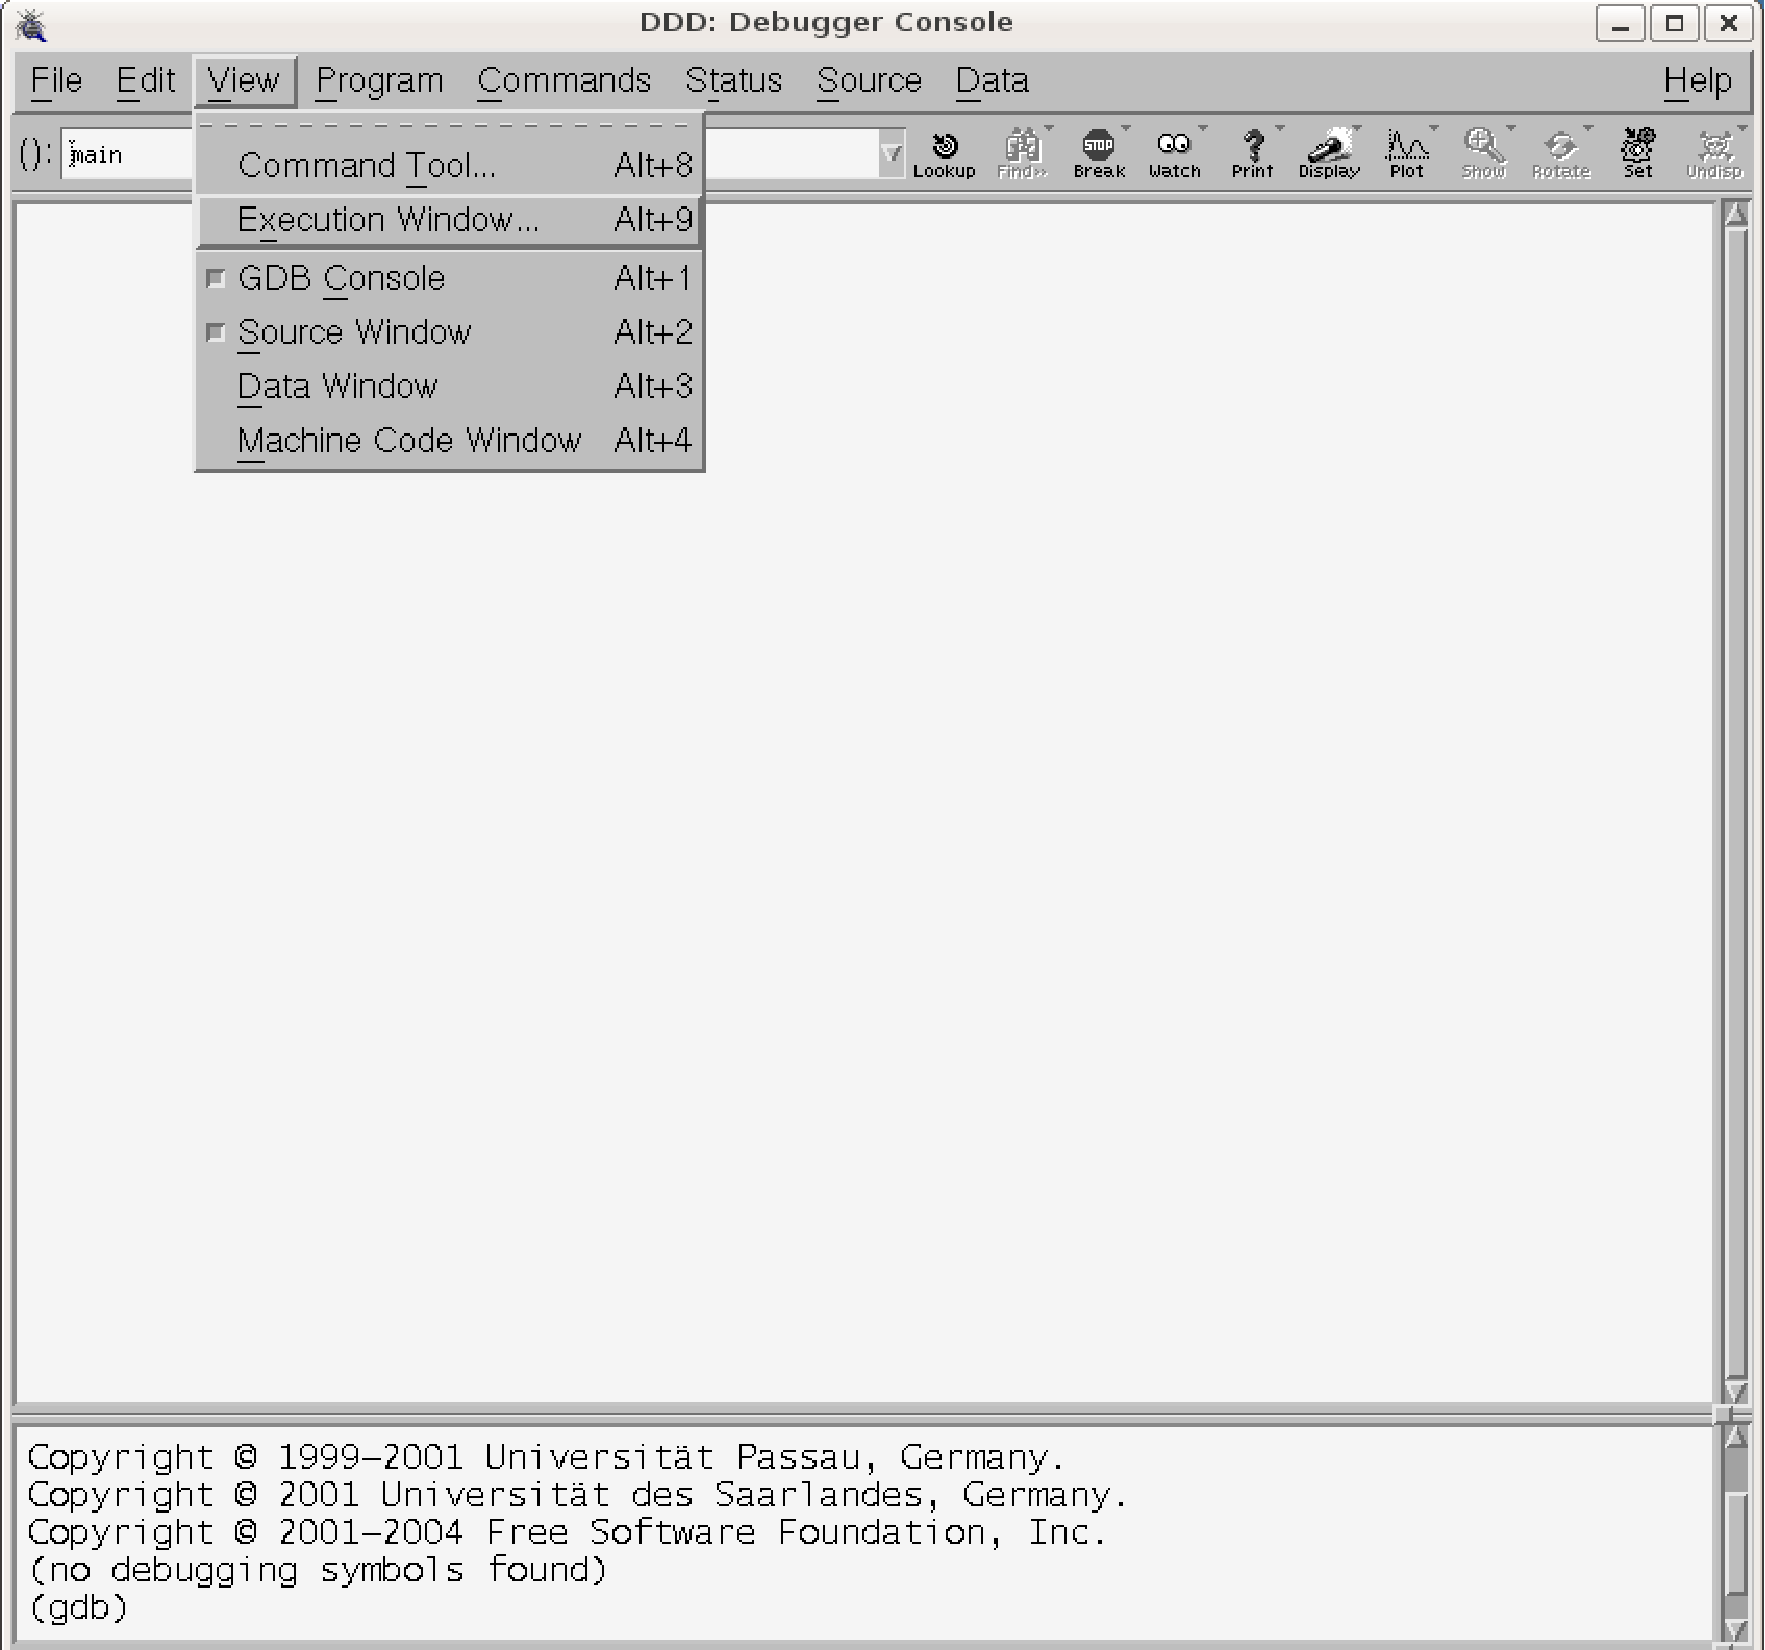
\includegraphics[width=8cm]{chapters/mardal-2/pdf/fig1.pdf}} \\
  \subfigure{ 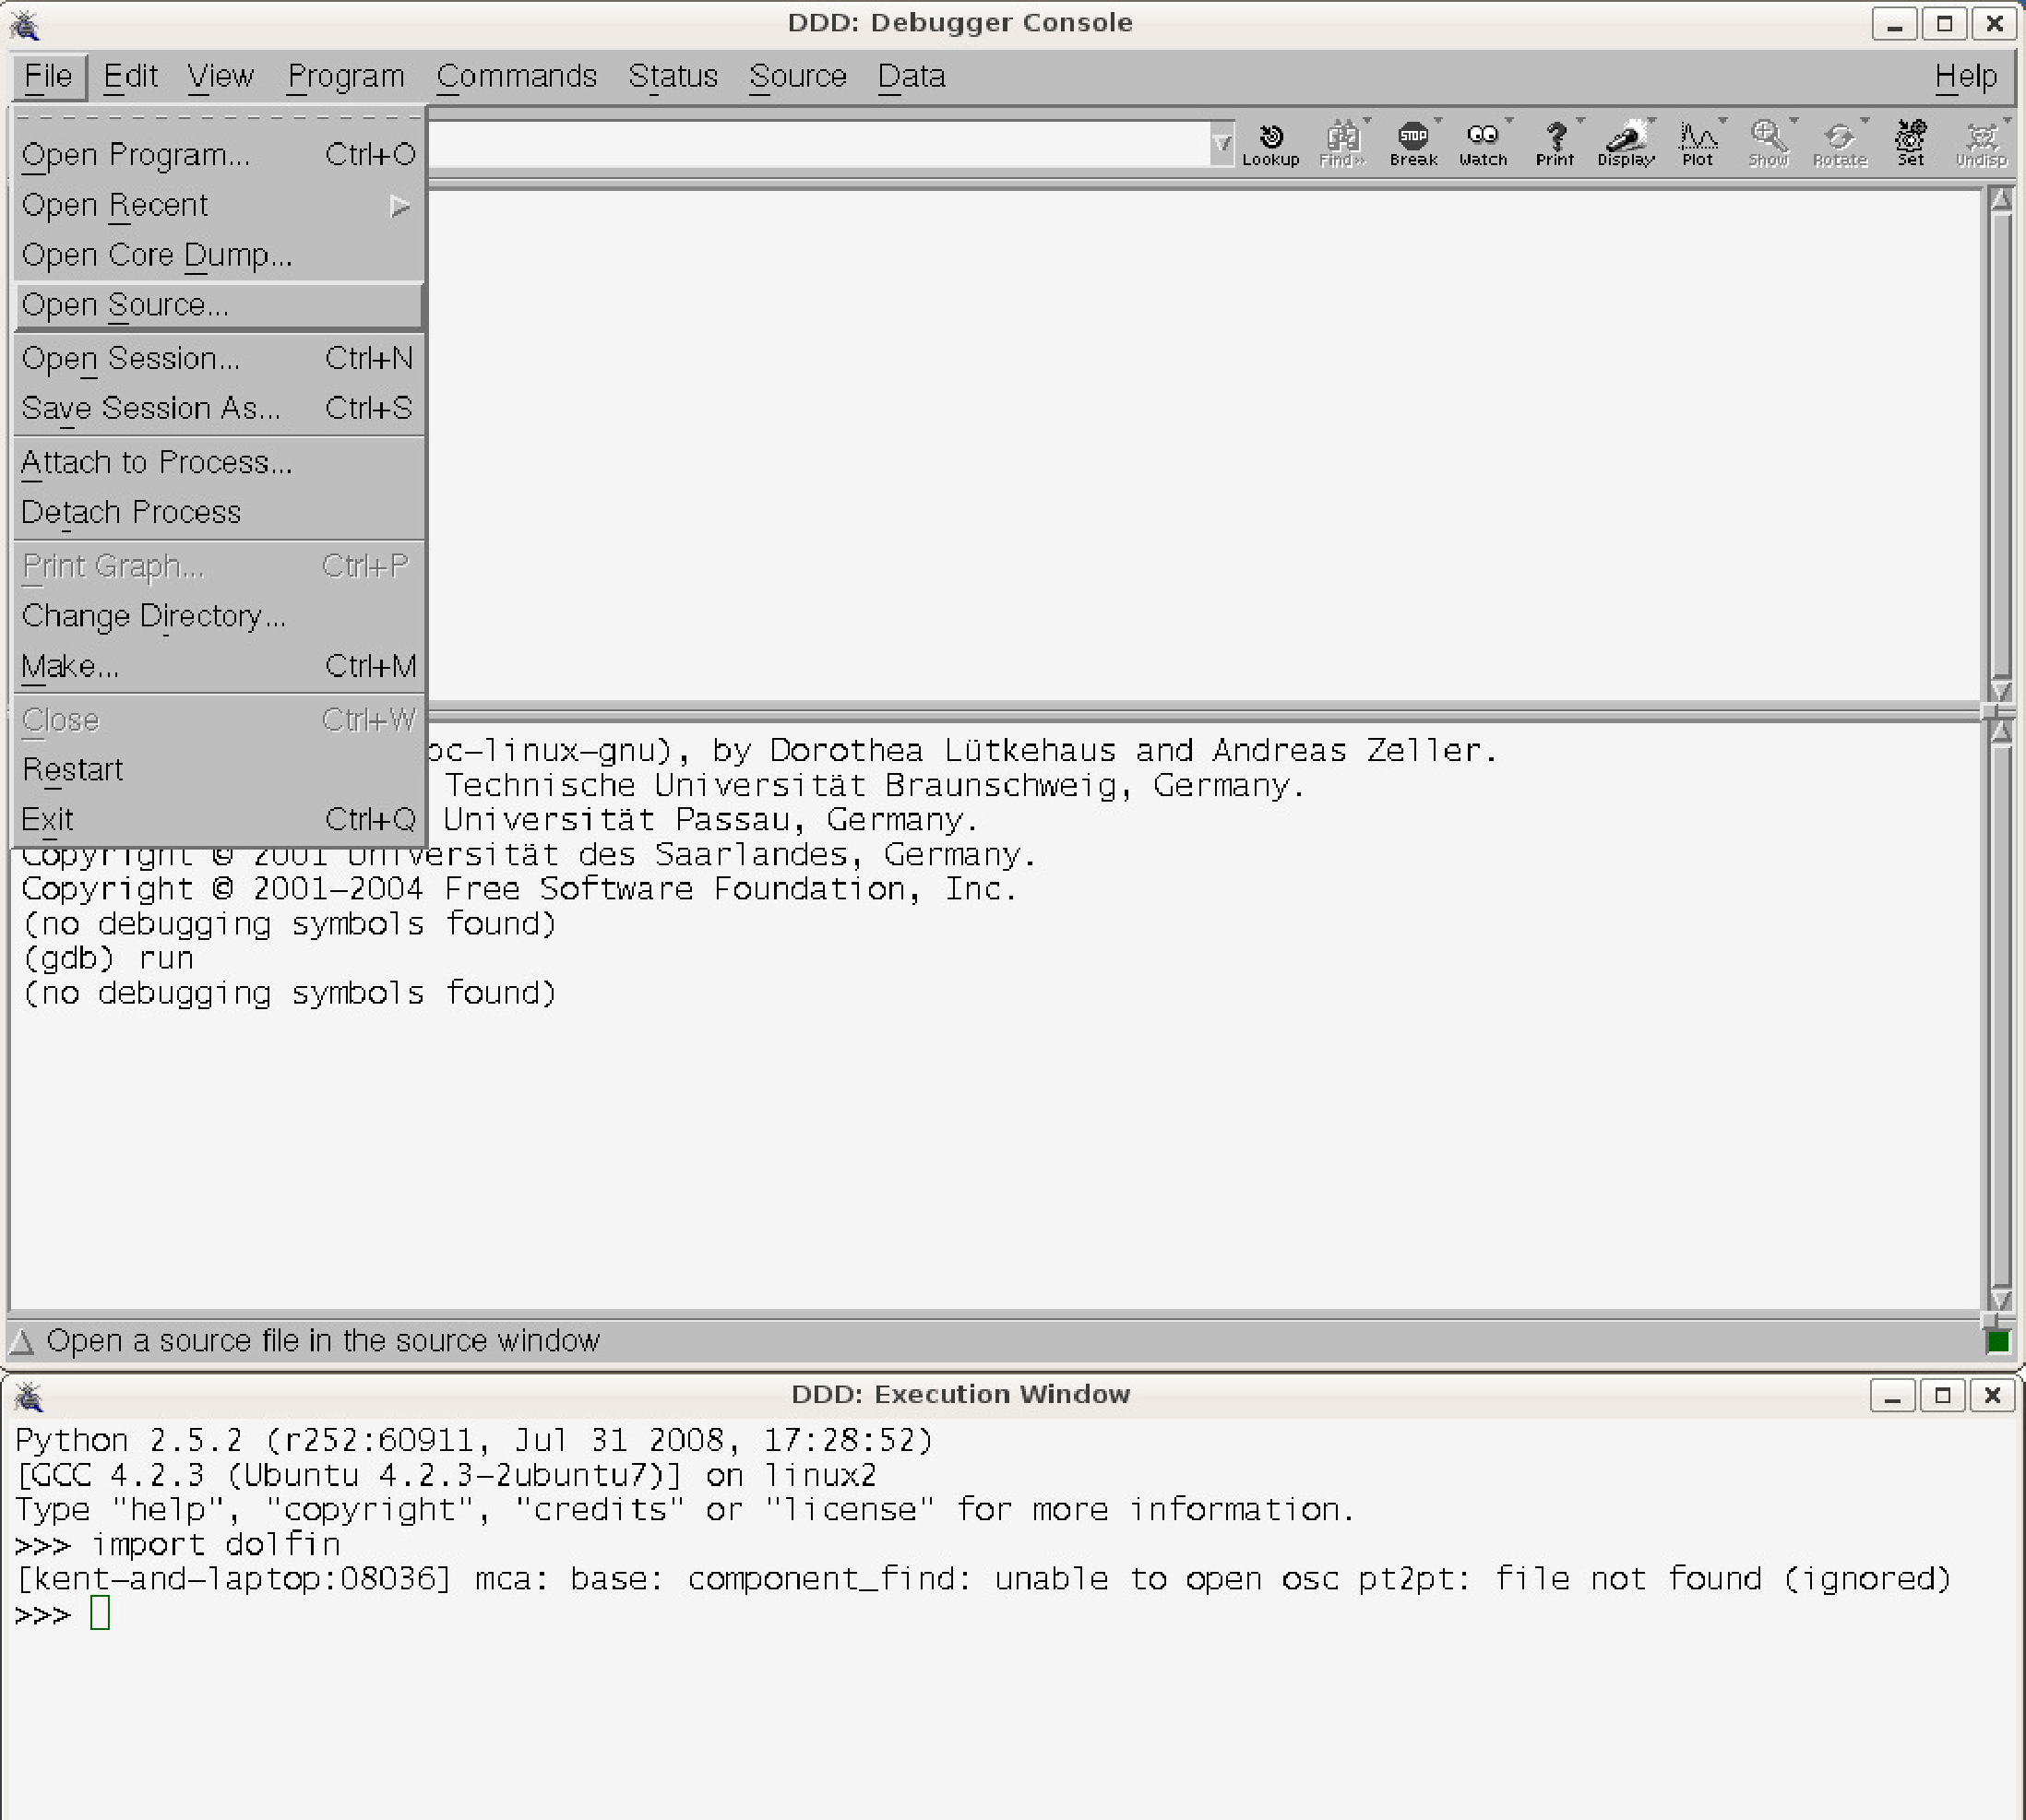
\includegraphics[width=8cm]{chapters/mardal-2/pdf/fig2.pdf}}
  \caption{Upper Picture: Starting a separate thread for the Python session in ddd.
           Lower Picture: Opening the source code after the \dolfin library has been loaded into Python.}
  \label{figure12}
\end{figure}
\begin{figure}
  \subfigure{ 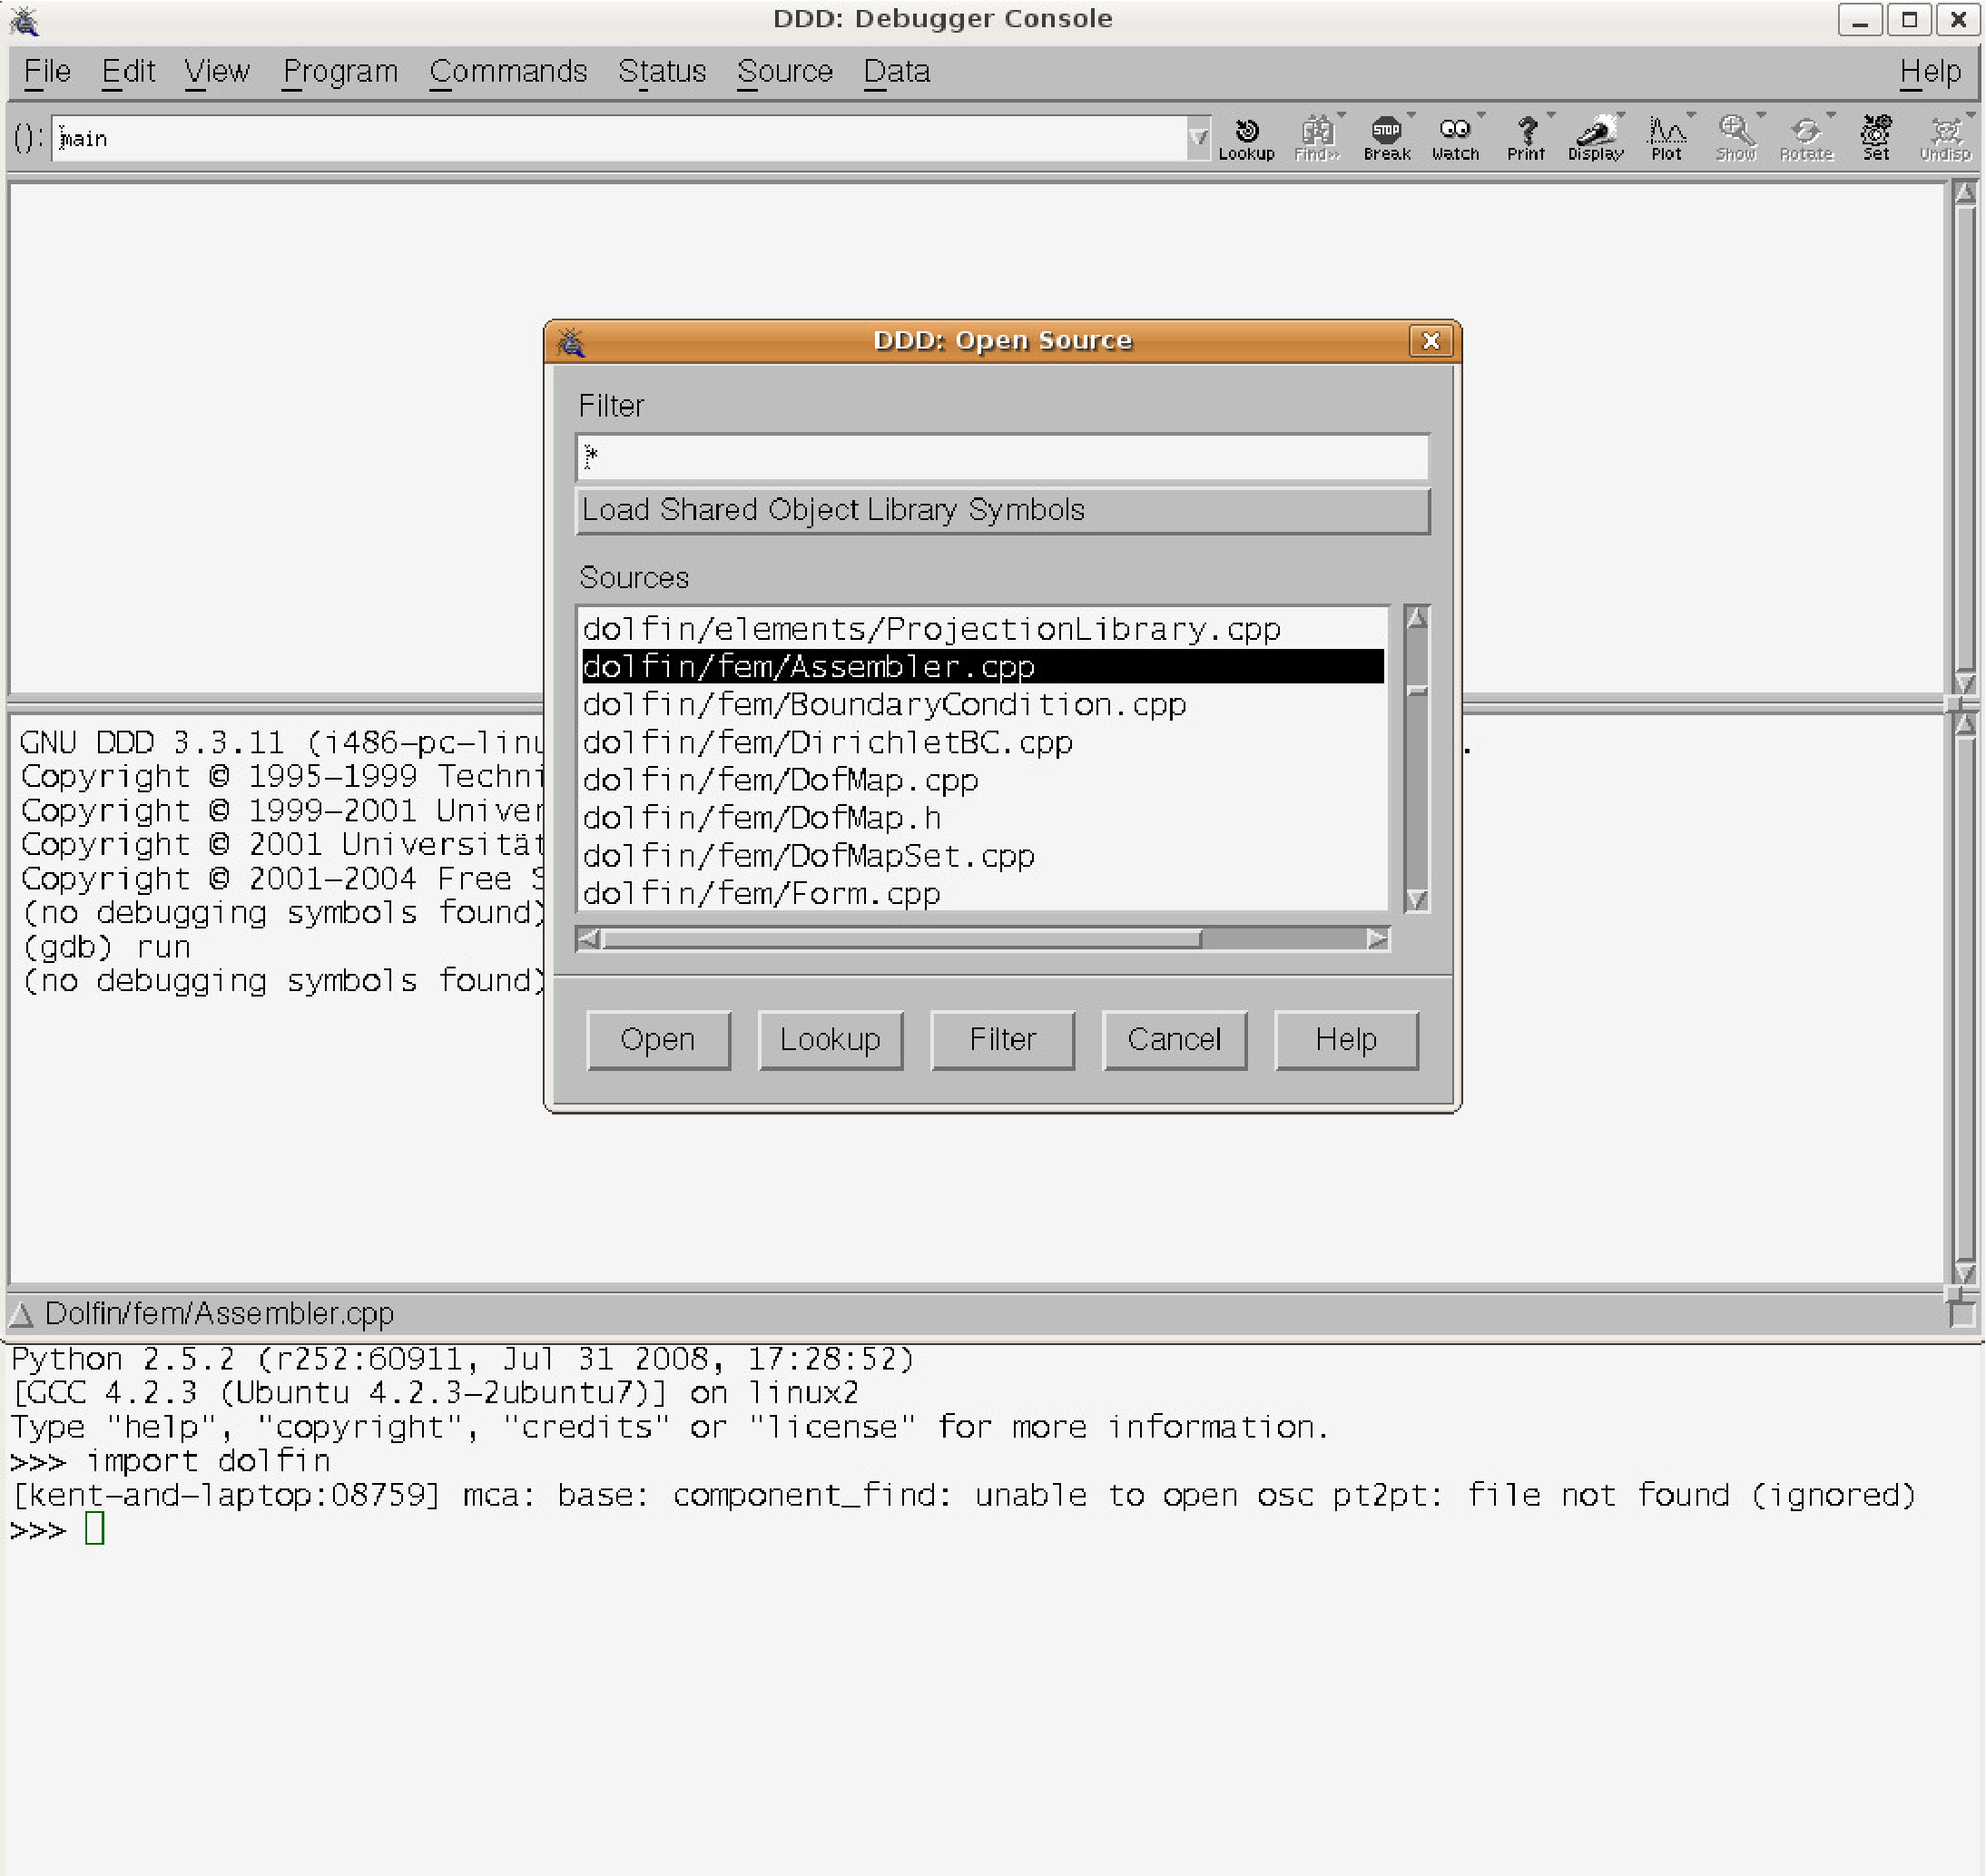
\includegraphics[width=8cm]{chapters/mardal-2/pdf/fig3.pdf}} \\
  \subfigure{ 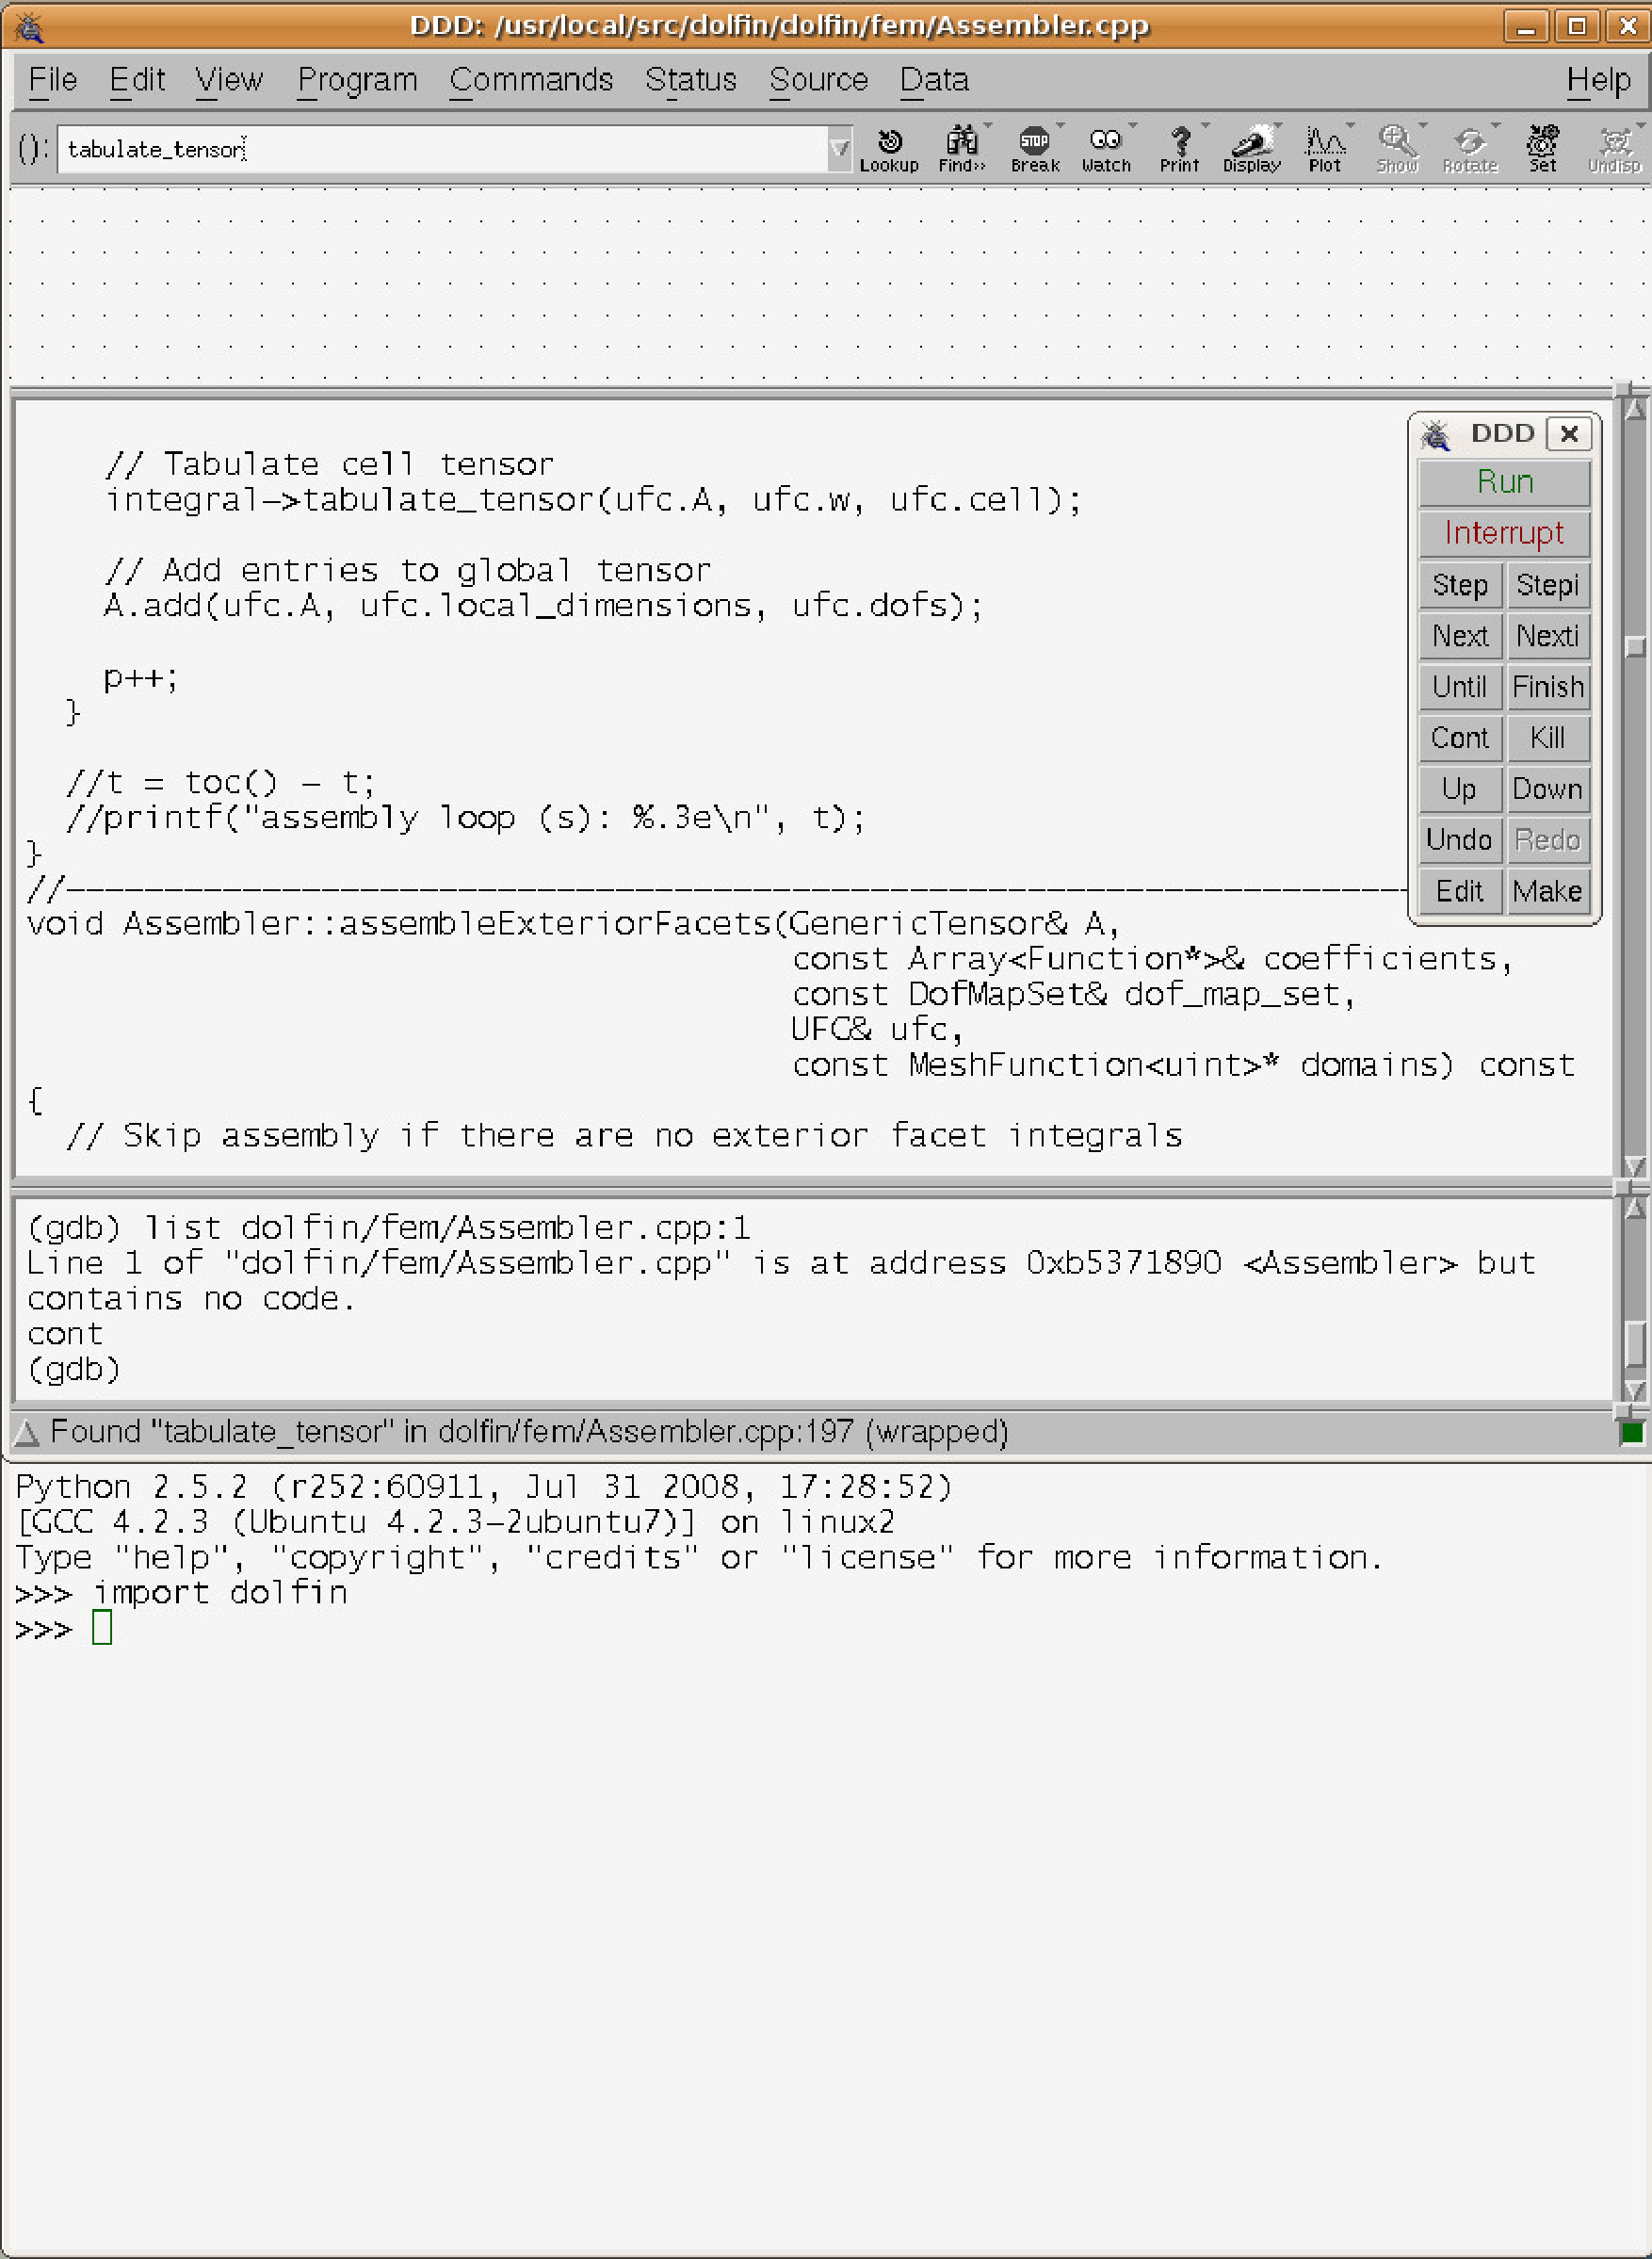
\includegraphics[width=8cm]{chapters/mardal-2/pdf/fig4.pdf}}
\caption{Upper Picture: Navigating through the source code for finding the assembly loop.
         Lower Picture: Searching for the function \emp{tabulate\_tensor.} }
\label{figure34}
\end{figure}

\begin{figure}
  \subfigure{ 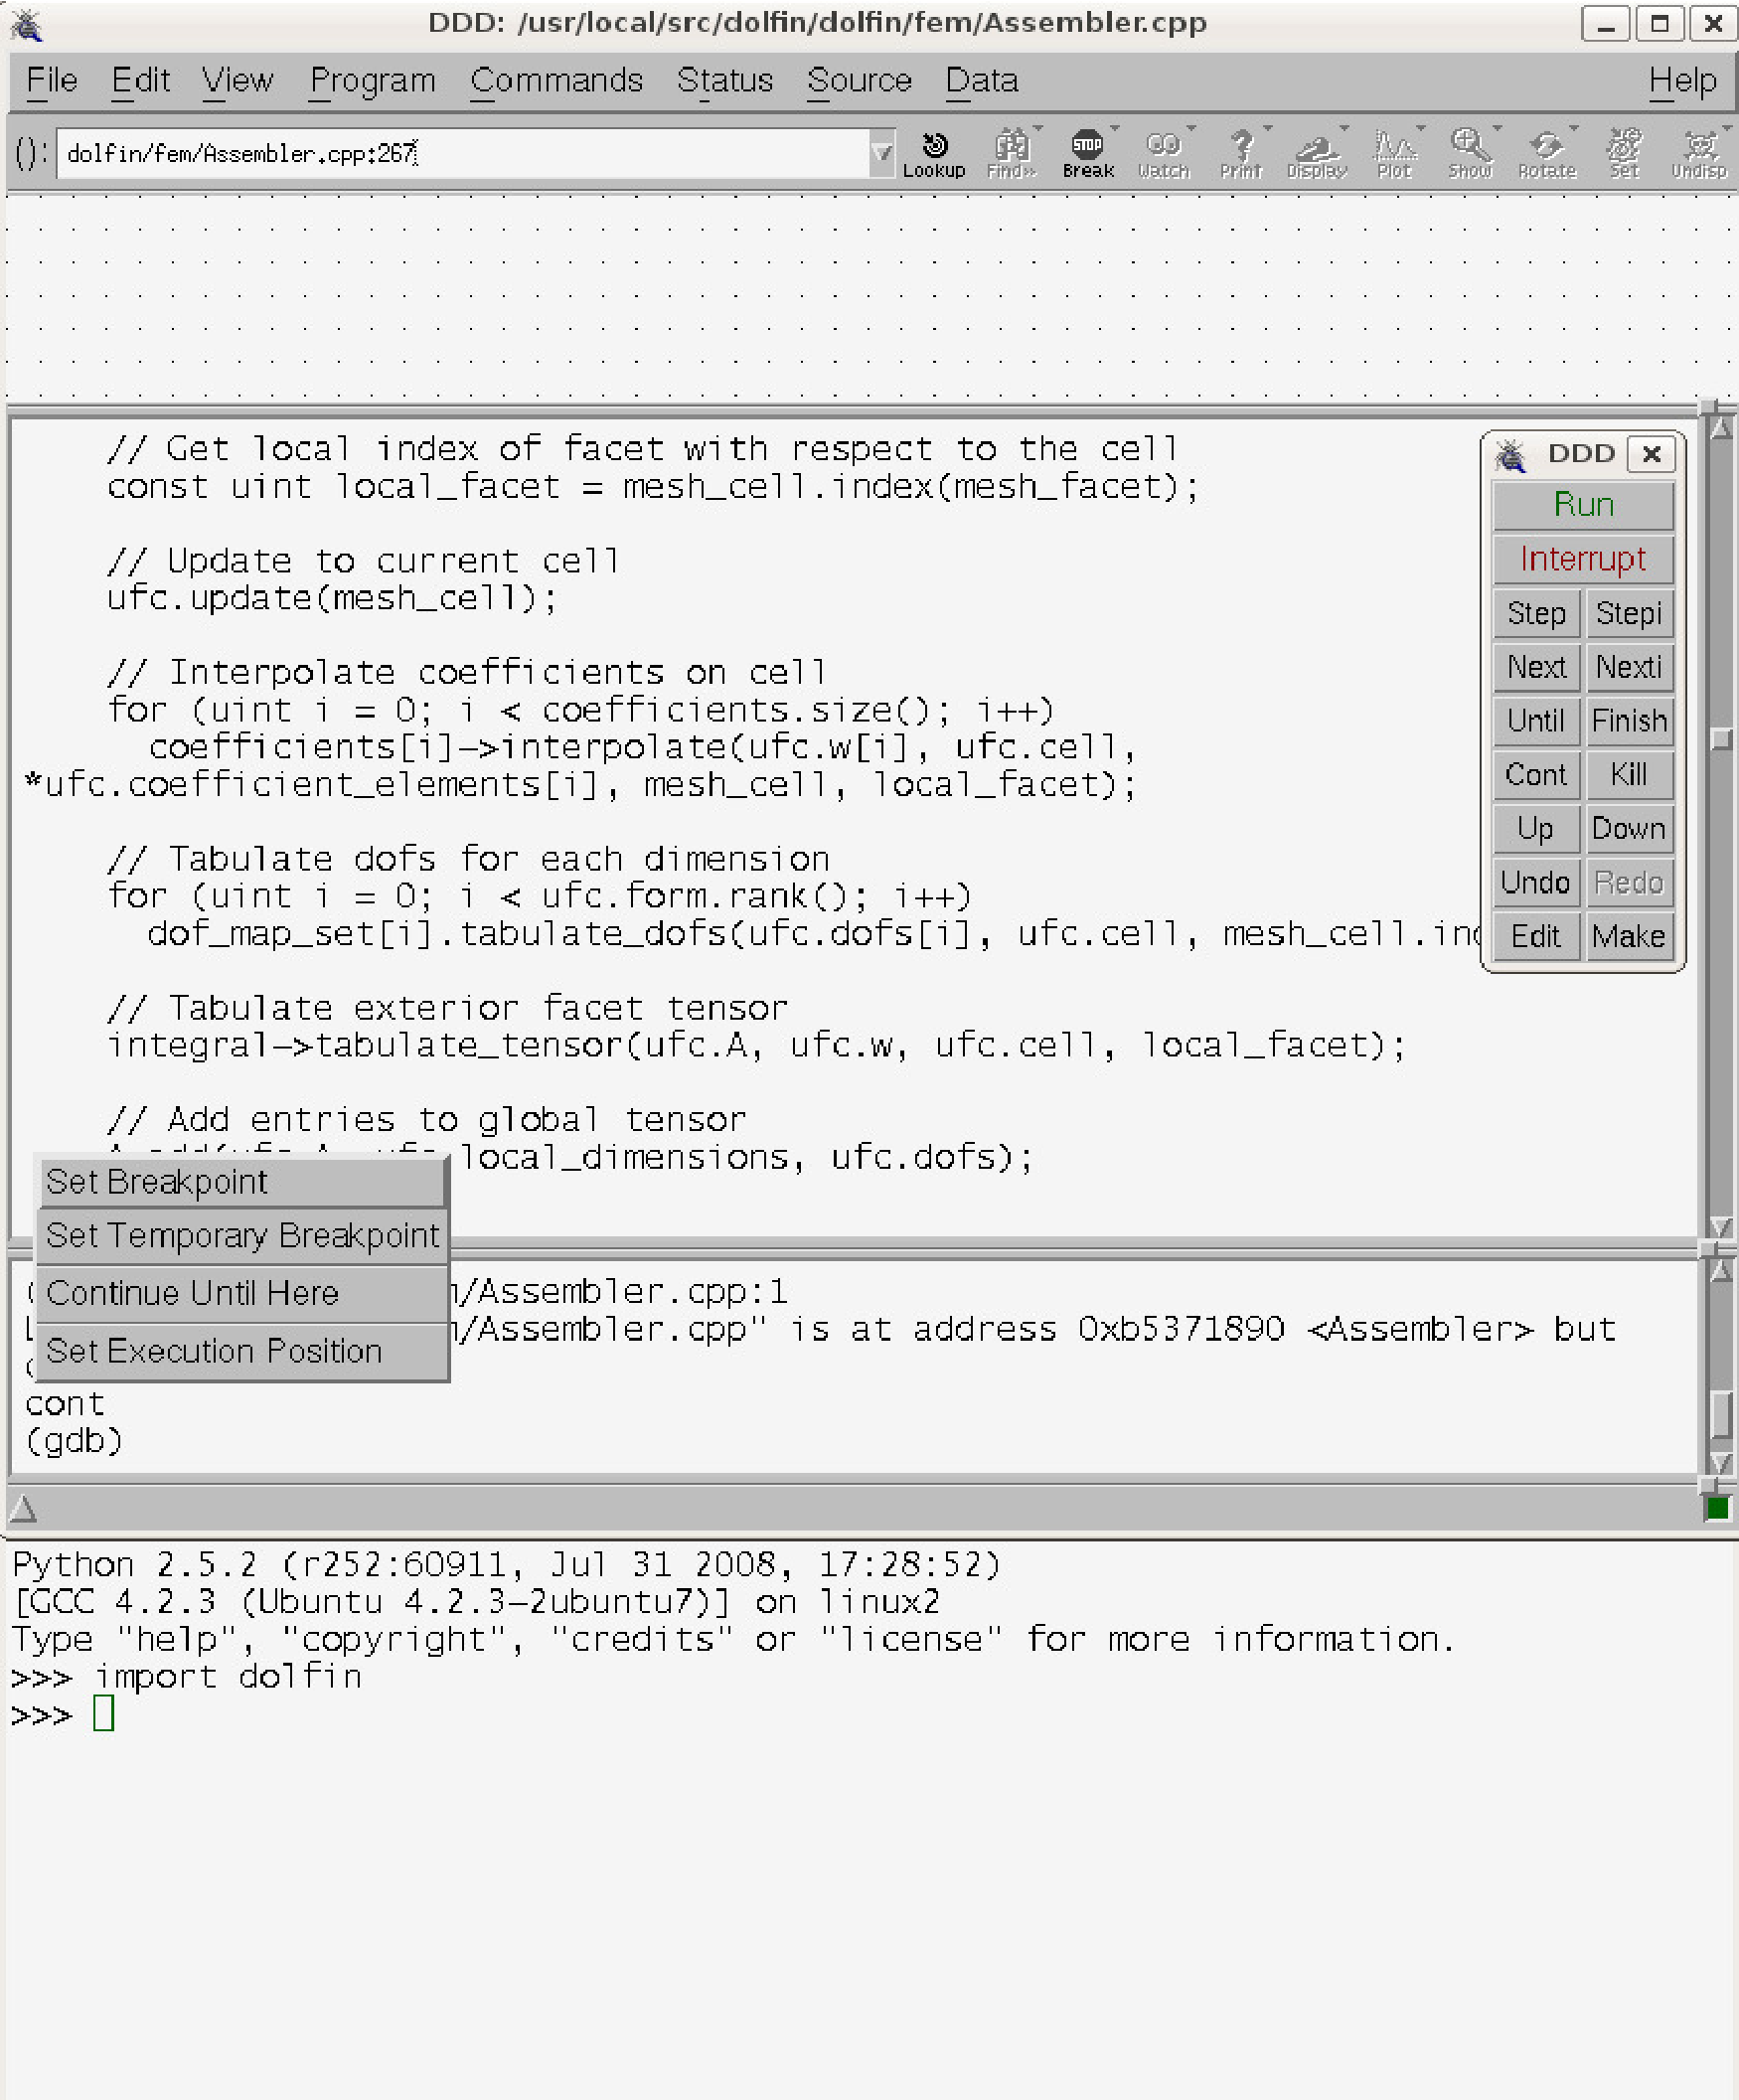
\includegraphics[width=8cm]{chapters/mardal-2/pdf/fig5.pdf}} \\
  \subfigure{ 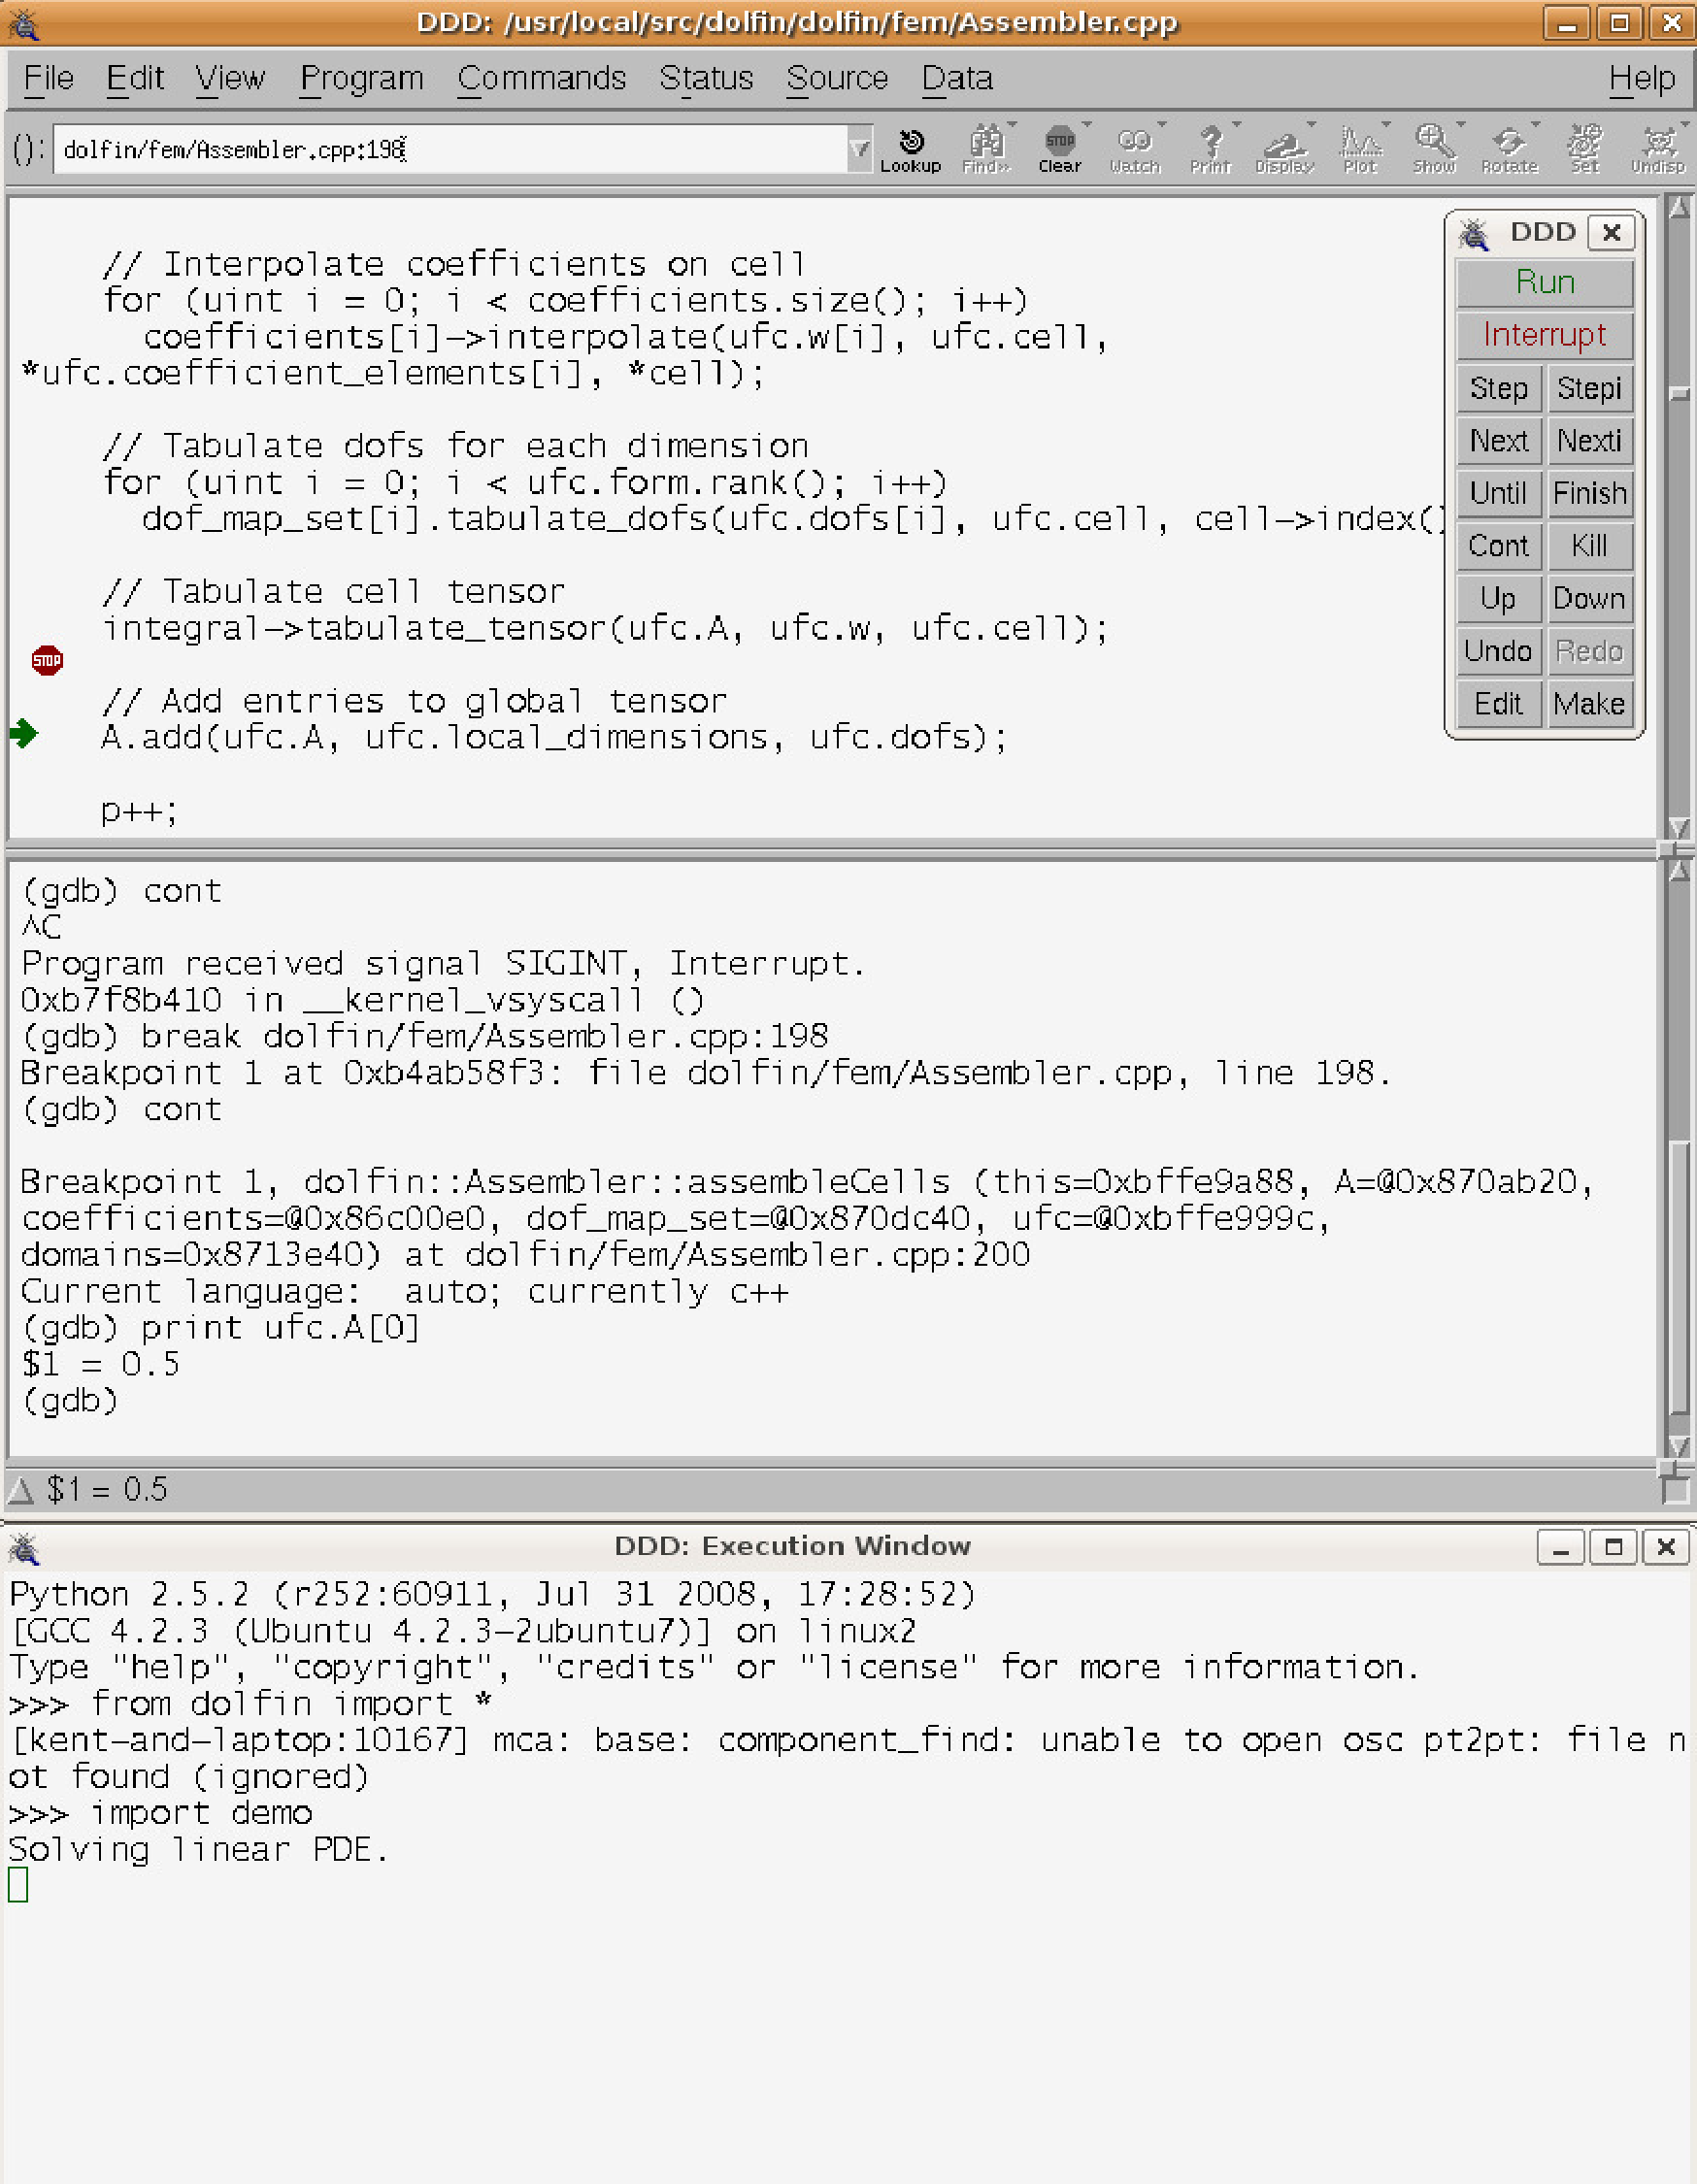
\includegraphics[width=8cm]{chapters/mardal-2/pdf/fig6.pdf}}
\caption{Setting a breakpoint after tabulate tensor and printing out the first element matrix entry.}
\label{fig5}
\end{figure}


%%% Local Variables:
%%% mode: latex
%%% TeX-master: "../../book"
%%% End:
